\chapter[Использование функций при программировании на \Sys{C++}]{Использование функций при программировании на \Sys{C++}}\label{ch04}
В практике программирования часто складываются ситуации, когда одну и ту же группу операторов, реализующих определённую
цель, требуется повторить без изменений в нескольких местах программы. Для избавления от столь нерациональной траты
времени была предложена концепция подпрограммы.

\index{Подпрограмма}\emph{Подпрограмма} --- именованная, логически законченная группа операторов языка,
которую можно вызвать для выполнения любое количество раз из различных мест программы. В языке \Sys{C++} подпрограммы
реализованы в виде \index{Функция}\emph{функций}~\cite{KR}.

\section[Общие сведения о функциях]{Общие сведения о функциях. Локальные и
глобальные переменные}
\index{Функция}\emph{Функция} --- это поименованный набор описаний и операторов, выполняющих определённую
задачу. Функция может принимать параметры и возвращать значение. Информация, передаваемая в функцию для обработки,
называется \emph{параметром}, а результат вычисления функции её \emph{значением}. Обращение к
функции называют \emph{вызовом}. Как известно (п.~\ref{ch02:8}), любая программа на \Sys{C++} состоит из одной или
нескольких функций. При запуске программы первой выполняется функция \Sys{main}. Если среди операторов
функции \Sys{main} встречается вызов функции, то управление передаётся операторам функции. Когда все
операторы функции будут выполнены, управление возвращается оператору, следующему за вызовом функции.

Перед вызовом функция должна быть обязательно описана. \index{Функция!описание}\emph{Описание функции}
состоит из заголовка и тела функции:
\begin{lstlisting}
`\Sys{тип имя\_функции(список\_переменных)}`
{
  `\Sys{тело\_функции}`
}
\end{lstlisting}
\index{Функция!заголовок}\emph{Заголовок функции} содержит:

\begin{itemize}
\item \Sys{тип} возвращаемого функцией значения, он может быть любым; если функция не возвращает значения,
указывают тип \Sys{void};
\item \Sys{имя\_функции;}
\item \Sys{список\_переменных} --- перечень передаваемых в функцию величин (\emph{аргументов}),
которые отделяются друг от друга запятыми; для каждой переменной из списка указывается \Sys{тип} и
\Sys{имя}; если функция не имеет аргументов, то в скобках указывают либо тип \Sys{void}, либо
ничего.
\end{itemize}
\index{Функция!тело функции}\emph{Тело функции} представляет собой последовательность описаний и
операторов, заключённых в фигурные скобки.

В общем виде \emph{структура программы} на \Sys{C++} может иметь вид:
\begin{lstlisting}
`\Sys{директивы компилятора}`
`\Sys{тип имя\_1(список\_переменных)}`
{
  `\Sys{тело\_функции\_1;}`
}

`\Sys{тип имя\_2(список\_переменных)}`
{
  `\Sys{тело\_функции\_2;}`
}

`\Sys{...}`

`\Sys{тип имя\_n(список\_переменных)}`
{
  `\Sys{тело\_функции\_n;}`
}

int main(`\Sys{список\_переменных}`)
{
  //`Тело функции может содержать операторы вызова функций \Sys{имя\_1, имя\_2, ..., имя\_n}`
  `\Sys{тело\_основной\_функции;}`
}
\end{lstlisting}
Однако допустима и другая \emph{форма записи программного кода}:

\begin{lstlisting}
`\Sys{директивы компилятора}`
`\Sys{тип имя\_1(список\_переменных);}`
`\Sys{тип имя\_2(список\_переменных);}`
`\Sys{...}`
`\Sys{тип имя\_n(список\_переменных);}`
int main(`\Sys{список\_переменных}`)
{
  //`Тело функции может содержать операторы вызова функций \Sys{имя\_1, имя\_2, ..., имя\_n}`
  `\Sys{тело\_основной\_функции;}`
}
`\Sys{тип имя\_1(список\_переменных)}`
{
  `\Sys{тело\_функции\_1;}`
}

`\Sys{тип имя\_2(список\_переменных)}`
{
  `\Sys{тело\_функции\_2;}`
}

`\Sys{...}`

`\Sys{тип имя\_n(список\_переменных)}`
{
  `\Sys{тело\_функции\_n;}`
}
\end{lstlisting}

Здесь функции описаны после функции \Sys{main()}, однако до неё перечислены заголовки всех функций. Такого
рода опережающие заголовки называют \index{Функция!прототип}\emph{прототипами
функций}. Прототип указывает компилятору тип данных, возвращаемых функцией, тип переменных,
выступающих в роли аргументов, и порядок их следования. Прототипы используются для проверки правильности вызова функций
в основной программе. Имена переменных, указанные в прототипе функции, компилятор игнорирует:
\begin{lstlisting}
//`Записи равносильны.`
int func(int a,int b);
int func(int ,int);
\end{lstlisting}

\index{Функция!вызов}\emph{Вызвать функцию} можно в любом месте программы. Для \emph{вызова
функции} необходимо указать её \Sys{имя} и в круглых скобках, через запятую перечислить
\Sys{имена} или \Sys{значения аргументов}, если таковые имеются:

\begin{lstlisting}
`\Sys{имя\_функции(список\_переменных);}`
\end{lstlisting}

Рассмотрим пример. Создадим функцию \Sys{f()}, которая не имеет входных значений и не формирует результат.
При вызове этой функции на экран выводится строка символов \Sys{"С Новым Годом, "}.

\begin{lstlisting}
#include <iostream>
using namespace std;
void f()  //`Описание функции.`
{
  cout << "`\Sys{С Новым Годом}`, ";
}
int main()
{
  f();      //`Вызов функции.`
  cout <<"`\Sys{Студент!}`" << endl;
  f();      //`Вызов функции.`
  cout <<"`\Sys{Преподаватель!}`" << endl;
  f();      //`Вызов функции.`
  cout <<"`\Sys{Народ!}`" << endl;
}
\end{lstlisting}

Результатом работы программы будут три строки:
\begin{verbatim}
С Новым Годом, Студент!
С Новым Годом, Преподаватель!
С Новым Годом, Народ!
\end{verbatim}

Далее приведён пример программы, которая пять раз выводит на экран фразу \Sys{"Здравствуй, мир!"}. Операция вывода строки символов оформлена в виде функции \Sys{fun()}. Эта функция также
не имеет входных значений и не формирует результат. Вызов функции осуществляется в цикле:
\begin{lstlisting}
#include <iostream>
using namespace std;
void fun()
{
  cout << "`\Sys{Здравствуй, мир}`!" << endl;
}

int main()
{
  for(int i=1;i<=5;fun(),i++);
}
\end{lstlisting}

Если тип возвращаемого значения не \Sys{void}, то функция может входить в состав выражений.
\emph{Типы и порядок следования переменных в определении и при вызове функции должны совпадать}. Для того
чтобы \index{Функция!возврат результата}\emph{функция вернула} какое-либо значение, в ней должен быть
оператор: 

\Sys{return (выражение);}

Далее приведён пример программы, которая вычисляет значение выражения  
$\sin^2(\alpha)+\cos^2(\alpha)$ при заданном значении  $\alpha$. Здесь функция \Sys{radian} выполняет
перевод градусной меры угла в радианную\footnote{Чтобы найти радианную меру какого-нибудь угла по заданной градусной
мере, нужно помножить число градусов на  $\frac{\pi}{180}$, число минут на  $\frac{\pi}{180\cdot 60}$, число секунд
на $\frac{\pi}{180\cdot 60\cdot 60}$ и найденные произведения сложить.}.
\begin{lstlisting}
#include <iostream>
#include <math.h>
#define PI 3.14159
using namespace std;
double radian(int deg, int min, int sec)
{
  return (deg*PI/180+min*PI/180/60+sec*PI/180/60/60);
}
int main()
{
  int DEG,MIN,SEC; double RAD;
  //`Ввод данных.`
  cout<<"Inpout:"<<endl;   //`Величина угла:`
  cout<<"DEG="; cin>>DEG;  //`градусы,`
  cout<<"MIN="; cin>>MIN;  //`минуты,`
  cout<<"SEC="; cin>>SEC;  //`секунды.`
  //`Величина угла в радианах.`
  RAD=radian(DEG,MIN,SEC); //`Вызов функции.`
  cout << "Value in radian A="<<RAD << endl;
  //`Вычисление значения выражения и его вывод.`
  cout << "sin(A)^2+cos(A)^2=";
  cout << pow(sin(RAD),2)+pow(cos(RAD),2) << endl;
  return 0;
}
\end{lstlisting}


Переменные, описанные внутри функции, а также переменные из списка аргументов, являются
\index{Переменная!локальная}\emph{локальными}. Например, если программа содержит пять разных функций, в
каждой из которых описана переменная $N$, то для \Sys{C++} это пять различных переменных. Область действия локальной переменной
не выходит за рамки функции. Значения локальных переменных между вызовами одной и той же функции не сохраняются. 

Переменные, определённые до объявления всех функций и доступные всем функциям, называют
\index{Переменная!глобальная}\emph{глобальными}. В функции глобальную переменную можно отличить, если не
описана локальная переменная с теми же именем.

Глобальные переменные применяют для передачи данных между функциями, но это затрудняет отладку программы. Для обмена
данными между функциями используют параметры функций и значения, возвращаемые функциями.

\section[Передача параметров в функцию]{Передача параметров в функцию}
Обмен информацией между вызываемой и вызывающей функциями осуществляется с помощью \index{Функция!механизм передачи
параметров}\emph{механизма передачи параметров}. \Sys{Список\_переменных}, указанный в
заголовке функции, называется \index{Функция!формальные параметры}\emph{формальными параметрами} или просто
\emph{параметрами} функции. \Sys{Список\_переменных} в операторе вызова функции --- это
\index{Функция!фактические параметры}\emph{фактические параметры} или \emph{аргументы}. 

\emph{Механизм передачи параметров обеспечивает замену формальных параметров фактическими параметрами} и
позволяет выполнять функцию с различными данными. Между фактическими параметрами в операторе вызова функции и
формальными параметрами в заголовке функции устанавливается взаимно однозначное соответствие.
\emph{Количество, типы и порядок следования формальных и фактических параметров должны совпадать}.

\index{Передача параметров}\emph{Передача параметров} выполняется следующим образом. Вычисляются выражения,
стоящие на месте фактических параметров. В памяти выделяется место под формальные параметры в соответствии с их
типами. Затем формальным параметрам присваиваются значения фактических. Выполняется проверка типов и при необходимости
выполняется их преобразование. %При несоответствии типов выдаётся диагностическое сообщение. 

Передача параметров в функцию может осуществляться \index{Передача параметров!по значению}\emph{по
значению} и \index{Передача параметров!по адресу}\emph{по адресу}. 

При передаче данных по значению функция работает с копиями фактических параметров, и доступа к исходным значениям
аргументов у неё нет. При передаче данных по адресу в функцию передаётся не переменная, а её адрес, и, следовательно,
функция имеет доступ к ячейкам памяти, в которых хранятся значения аргументов. Таким образом, данные, переданные по
значению, функция изменить не может, в отличие от данных, переданных по адресу. 

Если требуется запретить изменение параметра внутри функции, используют модификатор \Sys{const}. Заголовок
функции в общем виде будет выглядеть так:
\begin{lstlisting}
`\Sys{тип имя\_функции}`(const `\Sys{тип\_переменной* имя\_переменной, …)}`
\end{lstlisting}

Например:
\begin{lstlisting}
#include <iostream>
using namespace std;
int f1(int i)  //`Данные передаются по значению`
{
  return(i++);
}
int f2(int* j) //`Данные передаются по адресу. При подстановке фактического параметра,` 
               //`для получения его значения, применяется операция разадресации *`.
{
  return((*j)++);
}
int f3(const int* k)  //`Изменение параметра не предусмотрено`.
{
  return((*k)++);
}
int main()
{
  int a;
  cout<<"a=";cin>>a;
  f1(a);
  cout<<"a="<<a<<"\n";
  f2(&a); //`Для передачи фактического параметра используется операция взятия адреса \&`.
  cout<<"a="<<a<<"\n";
  f3(&a);
  cout<<"a="<<a<<"\n";
  return 0;
}
\end{lstlisting}

Результат работы программы:\\
\emph{Введено значение переменной a.}\\
\verb!a=5! \\
\emph{Значение переменной a после вызова функции f1 не изменилось.}\\
\verb!a=5! \\
\emph{Значение переменной a после вызова функции f2 изменилось.}\\
\verb!a=6! \\
\emph{Значение переменной a после вызова функции f3 не изменилось.}\\
\verb!a=6! 

Удобно использовать передачу данных по адресу, если нужно чтобы функция изменяла значения переменных в вызывающей
программе.

Далее приведён пример программы, в которой исходя из радианной меры  некоторого угла вычисляется величина смежного с ним
угла. На экран выводятся значения углов в градусной мере. Функция \Sys{degree} выполняет перевод из
радианной меры в градусную\footnote{Чтобы найти градусную меру угла по заданной радианной, нужно помножить число радиан
на  $\frac{180}{\pi }$; если из полученной дроби выделить целую часть, то получим градусы; если из числа полученного
умножением оставшейся дробной части на 60, выделить целую часть, получим минуты; секунды вычисляются аналогично из дробной
части минут.}. Эта функция ничего не возвращает. Её аргументами являются \emph{значение} переменной
\Sys{rad}, определяющее величину угла в радианах, и \emph{адреса} переменных
\Sys{deg}, \Sys{min}, \Sys{sec}, в которых будут храниться вычисленные
результаты --- градусная мера угла. 
\begin{lstlisting}
#include <iostream>
#include <math.h>
#define PI 3.14159
using namespace std;
void degree (double rad, int* deg, int* min, int* sec)
{
  *deg= floor(rad*180/PI);
  *min=floor((rad*180/PI-(*deg))*60);
  *sec=floor(((rad*180/PI-(*deg))*60-(*min))*60);
}
int main()
{
  int DEG,MIN,SEC; double RAD;
  cout<<"Inpout:"<<endl;
  cout << "Value in radian A=";cin>>RAD;
  degree(RAD,&DEG,&MIN,&SEC);
  cout << DEG<<" "<<MIN<<" "<<SEC << endl;
  degree(PI-RAD,&DEG,&MIN,&SEC);
  cout << DEG<<" "<<MIN<<" "<<SEC << endl;
return 0;
}
\end{lstlisting}

\section[Возврат результата с помощью оператора return]{Возврат результата с помощью оператора return}
\index{Функция!возврат результата}\emph{Возврат результата} из функции в вызывающую её функцию
осуществляется оператором

\Sys{return выражение;}

Работает оператор следующим образом. Вычисляется значение \Sys{выражения}, указанного после
\Sys{return}, и преобразуется к типу возвращаемого функцией значения. Выполнение функции завершается, а
вычисленное значение передаётся в вызывающую функцию. Любые операторы, следующие в функции за оператором
\Sys{return}, игнорируются. Программа продолжает свою работу с оператора, следующего за оператором вызова
данной функции.

Оператор \Sys{return} может отсутствовать в функциях типа \Sys{void}, если возврат происходит
перед закрывающейся фигурной скобкой, и в функции \Sys{main}.

Также функция может содержать несколько операторов \Sys{return}, если это определено потребностями
алгоритма. Например, в следующей программе функция \Sys{equation} вычисляет корни квадратного уравнения.
Если $a=0$ (уравнение не является квадратным), то в программу передаётся значение равное
$-1$, если дискриминант отрицательный (уравнение не имеет действительных корней), то
1, а если положительный, то  вычисляются корни уравнения и в программу передаётся 0.
\begin{lstlisting}
#include <iostream>
#include <math.h>
using namespace std;
int equation( float a,float b,float c,float *x1,float *x2)
{ float D=b*b-4*a*c;
  if (a==0) return -1;
  else if (D<0) return 1;
       else 
       {
         *x1=(-b+sqrt(D))/2/a;
         *x2=(-b-sqrt(D))/2/a;
         return 0;
       }
}

int main()
{
  float A, B, C, X1, X2; int P;
  cout<<"Enter the coefficients of the equation:"<<endl;
  cout<<"A="; cin>>A;
  cout<<"B="; cin>>B;
  cout<<"C="; cin>>C;
  P=equation( A, B, C, &X1, &X2);
  if (P==-1)  cout<<"input Error"<<endl;
  else if (P==1)  cout<<"No real roots"<<endl;
       else  cout<<"X1="<<X1<<" X2="<<X2<<endl;
  return 0;
}
\end{lstlisting}

\section[Решение задач с использованием функций]{Решение задач с использованием функций}
Рассмотрим несколько задач с применением функций.

\prg{Вводится последовательность из $N$ целых чисел, найти среднее арифметическое
совершённых чисел и среднее геометрическое простых чисел последовательности.}{ch04:prg1}

Напомним, что целое число называется \emph{простым}, если оно делится нацело только на само себя и единицу.
Подробно алгоритм определения простого числа описан в задаче~\ref{ch03:prg15} (рис.~\ref{ch03:refDrawing31}). 
В этой задаче кроме простых чисел
фигурируют совершённые числа. Число называется \emph{совершённым}, если сумма всех делителей, меньших его
самого, равна этому числу. Алгоритм, с помощью которого можно определить делители числа, подробно рассмотрен 
в задаче~\ref{ch03:prg14} (рис.~\ref{ch03:refDrawing30}).

Для решения поставленной задачи понадобятся две функции: 
\begin{itemize}
\item \Sys{prostoe} --- определяет, является ли число простым, аргумент функции целое число
$N$; функция возвращает 1, если число простое и 0 --- в противном
случае.;

\item \Sys{soversh} --- определяет, является ли число совершённым; входной параметр целое число
$N$; функция возвращает 1, если число является совершённым и 0 --- в
противном случае.
\end{itemize}
\begin{lstlisting}
#include <iostream>
#include <math.h>
unsigned int prostoe(unsigned int N) //`Описание функции.`
{
  //`Функция определяет, является ли число простым.`
  int i,pr;
  for(pr=1,i=2;i<=N/2;i++)
  if (N%i==0) {pr=0;break;}
  return pr;
}
unsigned int soversh(unsigned int N) //`Описание функции.`
{
  `//Функция определяет, является ли число совершённым.`
  unsigned int i,S;
  for(S=0,i=1;i<=N/2;i++)
    if (N%i==0) S+=i; 	//`Сумма делителей.`
  if (S==N) return 1;
  else return 0;
}
using namespace std;
int main()
{
  unsigned int i,N,X,S,kp,ks;
  long int P;
  cout <<"N="; cin>>N;
  for(kp=ks=S=0,P=1,i=1;i<=N;i++)
  {
    cout <<"X="; cin >> X; //`Вводится элемент последовательности.`
    if (prostoe(X))  // `X --- простое число.`		
    {
      kp++;  //`Счётчик простых чисел.`
      P*=X;  //`Произведение простых чисел.`
    }
    if (soversh(X)) //`X --- совершённое число.`
    {
      ks++;  //`Счётчик совершённых чисел.`
      S+=X;  //`Сумма совершённых чисел.`
    }
  }
  if (kp>0) //`Если счётчик простых чисел больше нуля,`
            //`считаем среднее геометрическое и выводим его,`
    cout<<"`\Sys{Среднее геометрическое}`="<<pow(P,(float) 1/kp)<<endl;
  else      //`в противном случае --– сообщение об отсутствии простых чисел.`
    cout<<"`\Sys{Нет простых чисел}`\n";
  if (ks>0) //`Если счётчик совершённых чисел больше нуля,` 
            //`считаем среднее арифметическое и выводим его,`
    cout<<"`\Sys{Среднее арифметическое}`="<<(float) S/ks<<endl;
  else    //`в противном случае --- сообщение об отсутствии совершённых чисел.`
    cout<<"`\Sys{Нет совершённых чисел}`\n";
return 0;
}
\end{lstlisting}

\prg{Вводится последовательность целых чисел, 0 --- конец последовательности. Найти
минимальное число среди простых чисел и максимальное --- среди чисел, не являющихся простыми.}{ch04:prg2}

Для решения данной задачи создадим функцию \Sys{prostoe}, которая будет проверять, является ли число
$N$ простым. Входным параметром функции будет целое положительное число $N$. Функция
будет возвращать значение $1$, если число простое, и $0$ --- в противном случае.
Алгоритм поиска максимума (минимума) подробно описан в задаче~\ref{ch03:prg20} (рис.~\ref{ch03:refDrawing33}).

Текст программы:
\begin{lstlisting}
#include <iostream>
using namespace std;
unsigned int prostoe(unsigned int N) 
{
  int i,pr;
  for(pr=1,i=2;i<=N/2;i++)
    if (N%i==0) {pr=0;break;}
  return pr;
}
int main()
{
  int kp=0,knp=0,min,max,N;
  for (cout << "N=", cin>>N; N!=0; cout<<"N=", cin>>N)
  //`В цикле вводится элемент последовательности` N.
    if (prostoe(N))  //N `--- простое число`,
    {
      kp++;  //`счётчик простых чисел.`
      if (kp==1) min=N;	//`Предполагаем, что первое простое число минимально,`
      else if (N<min) min=N; //`если найдётся меньшее число, сохраняем его.`
    }
    else  //N `--- простым не является,`
    {
      knp++;  //`счётчик чисел не являющихся простыми.`
      if (knp==1) max=N;  //`Предполагаем, что первое не простое число максимально,`
      else if (N>max) max=N; //`если найдётся большее число, сохраняем его.`
    }
    if (kp>0) //`Если счётчик простых чисел больше нуля,`
      cout <<"min= "<<min<<"\t";  //`выводим значение минимального простого числа,`
    else  //`в противном случае ---`	
      cout <<"`\Sys{Нет простых чисел}`"; //`сообщение об отсутствии простых чисел.`
      if (knp>0) //`Если счётчик чисел не являющихся простыми больше нуля,`
        cout <<"max="<<max<<endl; //`выводим значение максимального числа,`
      else //`в противном случае ---` 
        cout <<"`\Sys{Нет составных чисел}`";  //`сообщение об отсутствии чисел` 
	                          //`не являющихся простыми.`
  return 0;
}
\end{lstlisting}

\prg{Вводится последовательность из $N$ целых положительных чисел.
В каждом числе найти наименьшую и наибольшую цифры\protect\footnote{Выделение цифры из числа подробно 
описано в задаче~\ref{ch03:prg16}}.}{ch04:prg3}

Программный код к задаче~\ref{ch04:prg3}.
\begin{lstlisting}
#include <iostream>
using namespace std;
unsigned int Cmax(unsigned long long int P)
{
  unsigned int max;
  if (P==0) max=0;
  for (int i=1 ; P!=0;P/=10)
  {
    if (i==1) {max=P%10;i++;}
    if (P%10>max) max=P%10;
  }
  return max;
}
unsigned int Cmin(unsigned long long int P)
{
  unsigned int min;
  if (P==0) min=0;
  for (int i=1; P!=0;P/=10)
  {
    if (i==1) {min=P%10;i++;}
    if (P%10<min) min=P%10;
  }
  return min;
}
int main()
{
  unsigned int N, k;
  unsigned long long int X;
  for (cout<<"N=",cin>>N,k=1;k<=N;k++)
  {
    cout<<"X=";cin>>X;
    cout<<"`Максимальная цифра`="<<Cmax(X);
    cout<<"  `Минимальная цифра`="<<Cmin(X)<<endl;
  }
  return 0;
}
\end{lstlisting}

\prg{Вводится последовательность целых положительных чисел, 0 ---
конец последовательности. Определить, сколько в  последовательности чисел-палиндромов\protect\footnote{Палиндром --- любой
симметричный относительно своей середины набор символов.}.}{ch04:prg4}

Алгоритм определения палиндрома подробно описан в задаче~\ref{ch03:prg19}. 
Далее приведён программный код к задаче~\ref{ch04:prg4}

\begin{lstlisting}
#include <iostream>
using namespace std;
bool palindrom(unsigned long long int N)
{//`Функция определяет, является ли число $N$ палиндромом, возвращает \Sys{true}, если $N$ ---`
 //`палиндром, и \Sys{false} в противном случае`
  unsigned long int M,R,S; 
  int kol, i;
  for (R=1,kol=1,M=N;M/10>0; kol++,R*=10,M/=10);
  for(S=0,M=N,i=1;i<=kol;S+=M%10*R,M/=10,R/=10,i++);
    if (N==S) return true;
    else return false;
}
int main()
{ unsigned long long int X;
  int K;
  for (K=0,cout<<"X=",cin>>X;X!=0;cout<<"X=",cin>>X)
    if (palindrom(X)) K++;
    cout<<"`\Sys{Количество палиндромов равно}` K="<<K<<endl;
  return 0;
}
\end{lstlisting}

\prg{Заданы два числа --- $X$ в двоичной системе счисления,
$Y$ в системе счисления с основанием пять. Найти сумму этих чисел. Результат вывести в десятичной
системе счисления.}{ch04:prg5}

Любое целое число $N$, заданное в $b$-ичной системе счисления, можно представить в десятичной системе счисления: 
\begin{equation*}
N=P_n\cdot b^b+P_{n-1}\cdot b^{n-1}+...+P_2\cdot b^2+P_1\cdot b+P_0=\sum_{i=0}^n{P_i\cdot b^i},
\end{equation*}
где $b$ --- \emph{основание системы счисления} (целое положительное фиксированное число), 
$P_i$  --- \emph{разряд числа:} 
$0\leqslant P_i\leqslant b-1,i=0,1,2,...,n.$
Например,\\
$743_{10}=7\cdot 10^2+4\cdot 10^1+3\cdot 10^0=700+40+3=743_{10}$;\ \  
$1011101_2=1\cdot 2^6+0\cdot 2^5+1\cdot 2^4+1\cdot 2^3+1\cdot 2^2+0\cdot 2^1+1\cdot
2^0=64+16+8+4+1=93_{10}$.

Создадим функцию для перевода целого числа $N$, заданного в
$b$-ичной системе счисления, в десятичную систему счисления.

\begin{lstlisting}
#include <iostream>
using namespace std;
unsigned long long int DecNC(unsigned long long int N, unsigned int b)
{
//`Функция выполняет перевод числа` N, `заданного в `b`-ичной системе счисления,` 
//`в десятичную систему счисления`
  unsigned long long int S,P;
  for (S=0,P=1;N!=0;S+=N%10*P,P*=b,N/=10);
  return S;
}
int main()
{
  unsigned long long int X,Y; unsigned int bX,bY;
  cout<<"X=";cin>>X;  //`Ввод числа` X.
  cout<<"b=";cin>>bX; //`Ввод основания с/с.`
  cout<<"Y=";cin>>Y;  //`Ввод числа` X.
  cout<<"b=";cin>>bY; //`Ввод основания с/с.`
  //`Вывод заданных чисел в десятичной с/с.`
  cout<<X<<"("<<bX<<")="<<DecNC(X,bX)<<"(10)"<<endl;
  cout<<Y<<"("<<bY<<")="<<DecNC(Y,bY)<<"(10)"<<endl;
  //`Вычисление суммы и вывод результата.`
  cout<<X<<"("<<bX<<")+"<<Y<<"("<<bY<<")=";
  cout<<DecNC(X,bX)+DecNC(Y,bY)<<"(10)"<<endl;
  return 0;
}
\end{lstlisting}


\prg{Задано число $X$ в десятичной системе
счисления. Выполнить перевод числа в системы счисления с основанием 2, 5 и 7.}{ch04:prg6}

Вообще, для того чтобы перевести целое число из десятичной системы счисления в другую, необходимо выполнить следующие
действия:

\begin{enumerate}
\item Разделить данное число на основание новой системы счисления: остаток от деления --- младший разряд нового числа;
%\item перевести остаток от деления в новую систему счисления; получается младший разряд нового числа;
\item Если частное от деления не равно нулю, продолжать деление, как указано в п.1.
\end{enumerate}
На рис.~\ref{ch04:refDrawing0} 
%Ниже
приведён пример <<ручного>> перевода числа 256, заданного в десятичной системе 
счисления, в восьмеричную. В
результате получим  $256_{(10)}=400_{(8)}$.
\begin{figure}[h]
\begin{minipage}[b]{0.5\textwidth}
$$
\begin{array}{r@{\,}l|l@{\,}l@{\,}l|l}
256 && \multicolumn{4}{l}8\\\cline{3-4}
- 256 &&& \phantom{-}32 &&8\\\cline{1-1}\cline{6-6}
 0 &&& - 32 && 4 \\\cline{4-4}
  && \multicolumn{4}{c}0\\
\end{array}
$$
\caption{Пример перевода числа в новую систему счисления}
\label{ch04:refDrawing0}
\end{minipage}
\end{figure}

Далее приведён текст программы, реализующей решение задачи~\ref{ch04:prg6}.

\begin{lstlisting}
#include <iostream>
using namespace std;
unsigned long long int NC(unsigned long long int N, unsigned int b)
{
  unsigned long long int S,P;
  for (S=0,P=1;N!=0;S+=N%b*P,P*=10,N/=b);
    return S;
}
int main()
{
  unsigned long long int X;
  cout<<"X=";cin>>X;  //`Ввод числа` X.
  //`Перевод числа` X `в заданные системы счисления.`
  cout<<X<<"(10)="<<NC(X,2)<<"(2)"<<endl;
  cout<<X<<"(10)="<<NC(X,5)<<"(5)"<<endl;
  cout<<X<<"(10)="<<NC(X,7)<<"(7)"<<endl;
  return 0;
}
\end{lstlisting}

\prg{Найти корни уравнения  $x^2-\cos (5\cdot x)=0$.}{ch04:prg7}

Для
решения задачи использовать:
\begin{itemize}
\item \emph{метод половинного деления},
\item \emph{метод хорд},
\item \emph{метод касательных} (метод Ньютона),
\item \emph{метод простой итерации}.
\end{itemize}
Оценить степень точности предложенных \emph{численных методов}, определив, за сколько итераций был найден
корень уравнения. Вычисления проводить с точностью  $\varepsilon=10^{-3}$.

Вообще говоря, \emph{аналитическое решение уравнения}

\begin{equation}\label{ch04:refDrawing0a}
f(x)=0
\end{equation}
можно найти только для узкого класса функций. В большинстве случаев приходится решать уравнение (\ref{ch04:refDrawing0a})
\emph{численными методами}. Численное решение уравнения (\ref{ch04:refDrawing0a}) проводят в два этапа: сначала
необходимо \emph{отделить корни уравнения}, т.е. найти достаточно тесные промежутки, в которых содержится
только один корень, эти промежутки называют \emph{интервалами изоляции корня}; на втором этапе проводят
уточнение отделённых корней, т.е. \emph{находят корни с заданной точностью}.

Интервал можно выделить, изобразив график функции, или каким-либо другим способом. Но все способы основаны на следующем
свойстве непрерывной функции: если функция  $f(x)$  непрерывна на интервале  $[a,b]$ и на его концах имеет различные
знаки,  $f(a)\cdot f(b)<0$, то между точками имеется хотя бы один корень. Будем считать интервал настолько малым, что в
нём находится только один корень. Рассмотрим самый простой способ уточнения корней.

Графическое решение задачи~\ref{ch04:prg7} показано на рис.~\ref{ch04:refDrawing1}. 
Так как функция  $f(x)=x^2-\cos (5\cdot x)$
 дважды пересекает ось абсцисс, можно сделать вывод о наличии  в уравнении  $x^2-\cos (5\cdot x)=0$  двух корней.
Первый находится на интервале  $[-0.4;-0.2]$ , второй принадлежит отрезку  $[0.2;0.4]$ .

\begin{figure}[htb]
\begin{center}
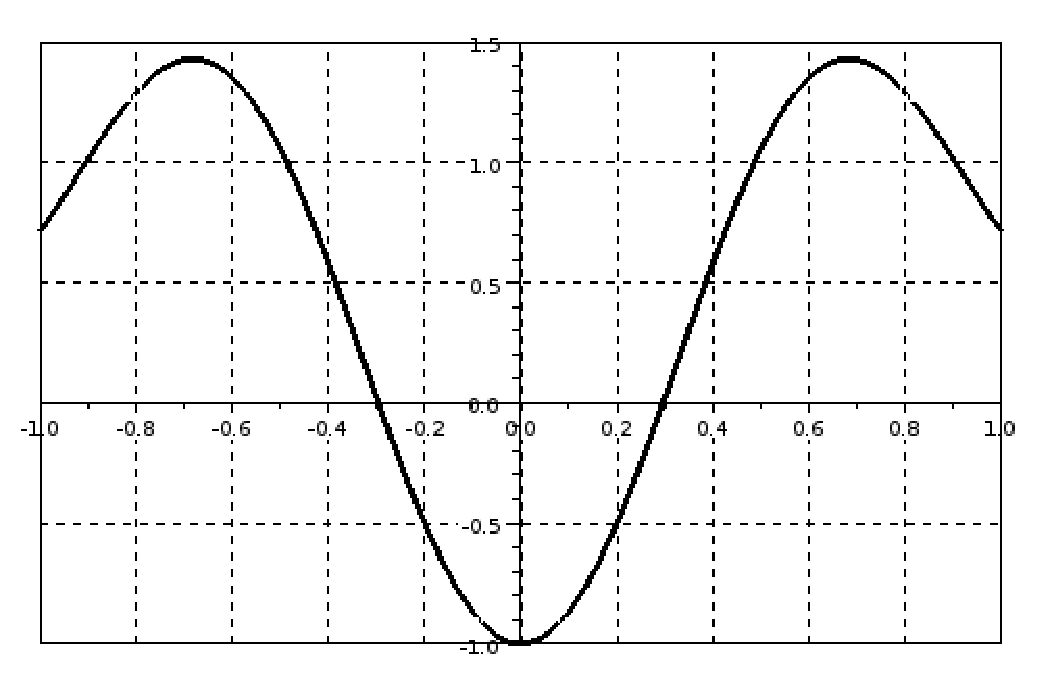
\includegraphics[width=0.5\textwidth]{img/ris_4_2}
\caption{Геометрическое решение задачи \ref{ch04:prg7}}
\label{ch04:refDrawing1}
\end{center}
\end{figure}

Рассмотрим предложенные в задаче \emph{численные методы} решения нелинейных уравнений.

\emph{Метод половинного деления (дихотомии)}. Пусть был выбран интервал изоляции  $[a,b]$  (рис.
\ref{ch04:refDrawing2}). Примем за первое приближение корня точку $c$, которая является серединой отрезка 
$[a,b]$ . Далее будем действовать по следующему алгоритму:
\begin{enumerate}
\item Находим точку  $c=\frac{a+b}{2}$;
\item Находим значение  $f(c)$;
\item Если  $f(a)\cdot f(c)<0$ , то корень лежит на интервале  $[a,c]$ , иначе корень лежит на интервале  $[c,b]$ ;
\item Если величина интервала меньше либо равна  $\varepsilon$, то найден корень с точностью  $\varepsilon$ , иначе
возвращаемся к~п.1.
\end{enumerate}

\begin{figure}[htb]
\begin{center}
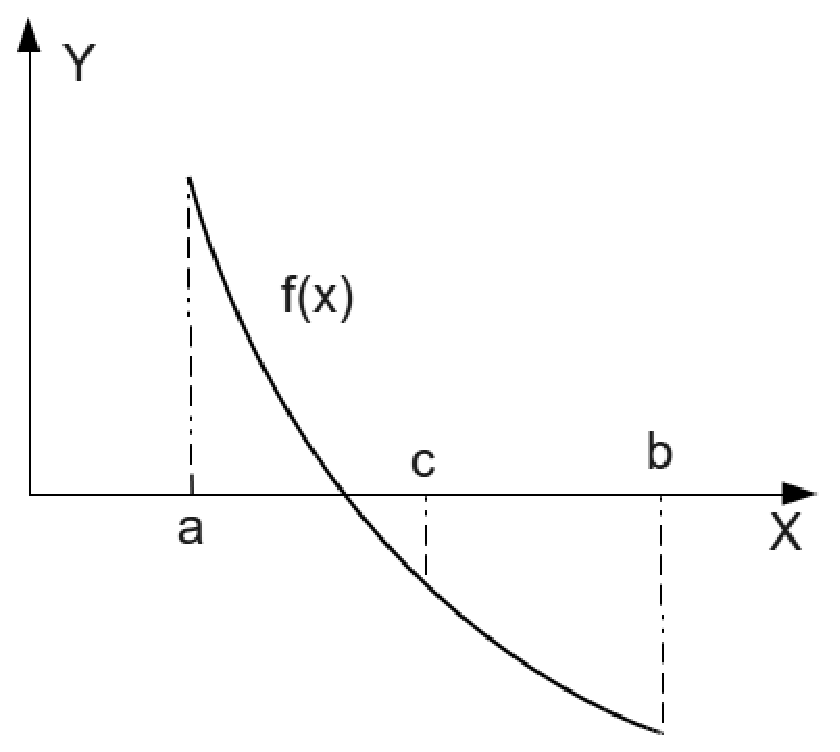
\includegraphics[width=0.5\textwidth]{img/ris_4_3}
\caption{Графическая интерпретация метода половинного деления}
\label{ch04:refDrawing2}
\end{center}
\end{figure}

Итак, для вычисления одного из корней уравнения  $x^2-\cos (5\cdot x)=0$  методом половинного деления достаточно знать
интервал изоляции корня  $a=0.2;b=0.4$  и точность вычисления  $\varepsilon=10^{-3}$ . 

Блок-схема алгоритма решения уравнения методом дихотомии приведена на рис.~\ref{ch04:refDrawing3}. 
Понятно, что здесь  $c$  --- корень заданного уравнения.

\begin{figure}[htb]
\begin{center}
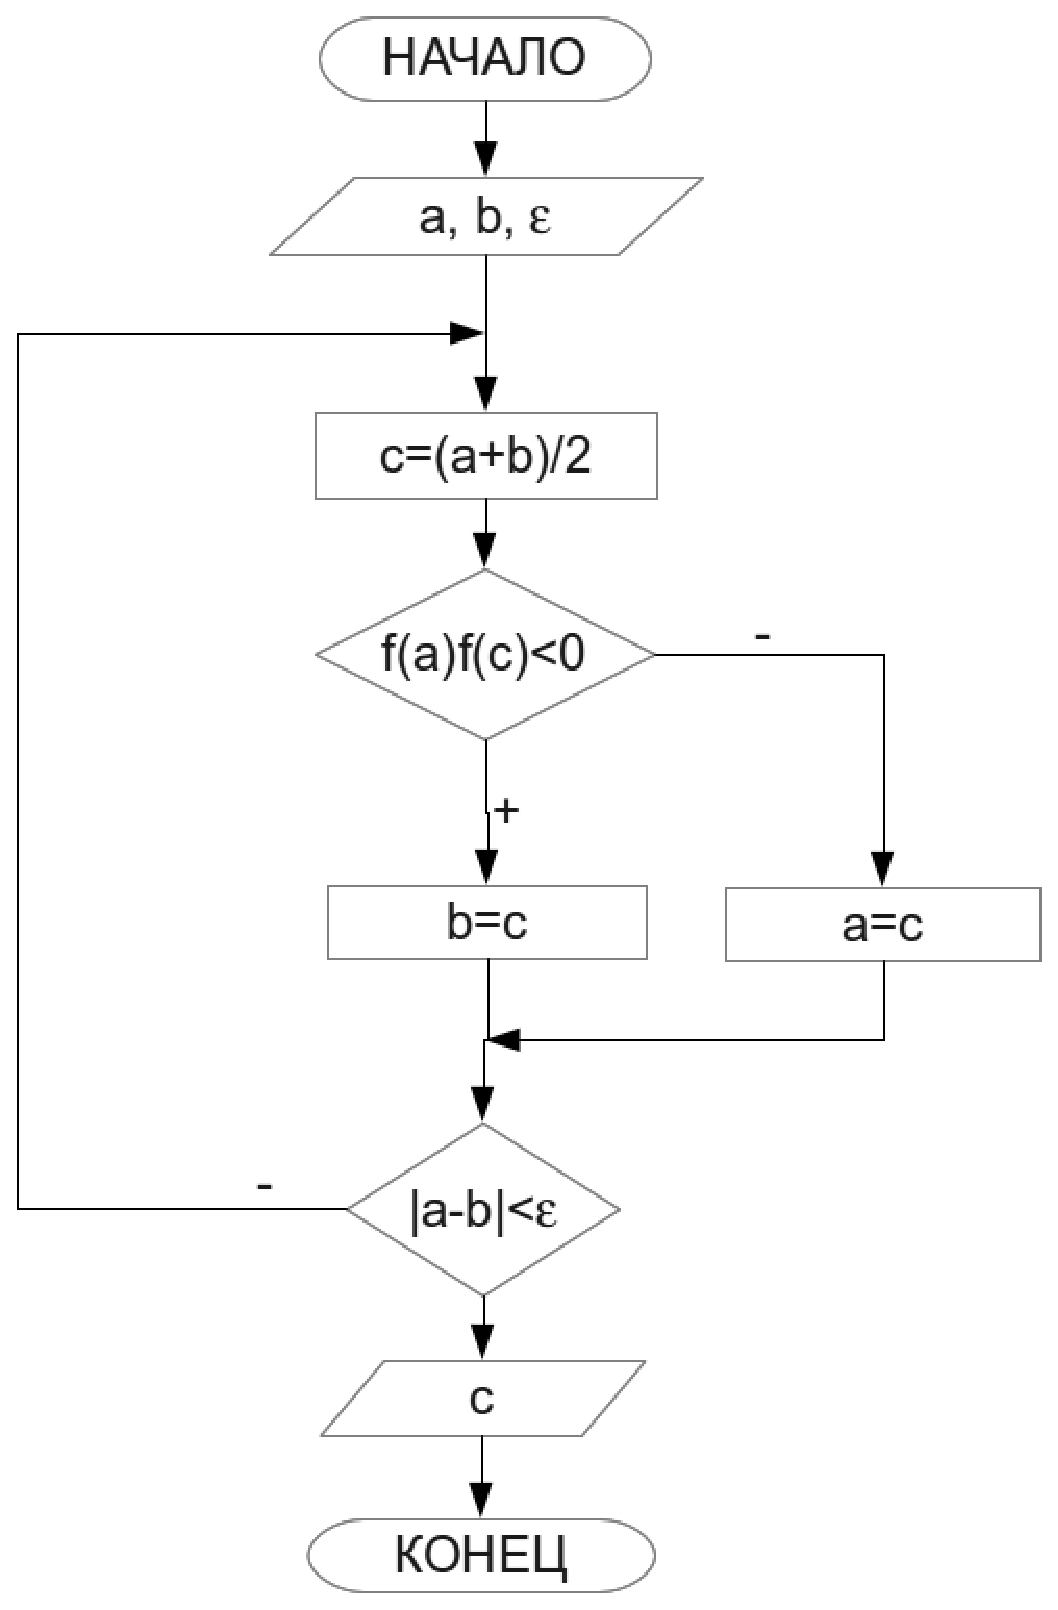
\includegraphics[width=0.5\textwidth]{img/ris_4_4}
\caption{Алгоритм решения уравнения методом дихотомии}
\label{ch04:refDrawing3}
\end{center}
\end{figure}

Однако, несмотря на простоту, такое последовательное сужение интервала проводится редко, так как требует слишком
большого количества вычислений. Кроме того, этот способ не всегда позволяет найти решение с заданной точностью.
Рассмотрим другие способы уточнения корня. При применении этих способов будем требовать, чтобы функция  $f(x)$ 
удовлетворяла следующим условиям на интервале  $[a,b]$ :
\begin{enumerate}
\item функция  $f(x)$  непрерывна вместе со своими производными первого и второго порядка. Функция  $f(x)$  на концах
интервала  $[a,b]$  имеет разные знаки  $f(a)\cdot f(b)<0$ ;
\item первая и вторая производные  $f'(x)$  и  $f''(x)$ сохраняют определённый
знак на всём интервале  $[a,b]$ .
\end{enumerate}

\emph{Метод хорд}. Этот метод отличается от метода дихотомии тем, что очередное приближение берём не в
середине отрезка, а в точке пересечения с осью $X$ (рис.~\ref{ch04:refDrawing4}) прямой, соединяющей точки 
$(a,f(a))$ и  $(b,f(b))$.

\begin{figure}[htb]
\begin{center}
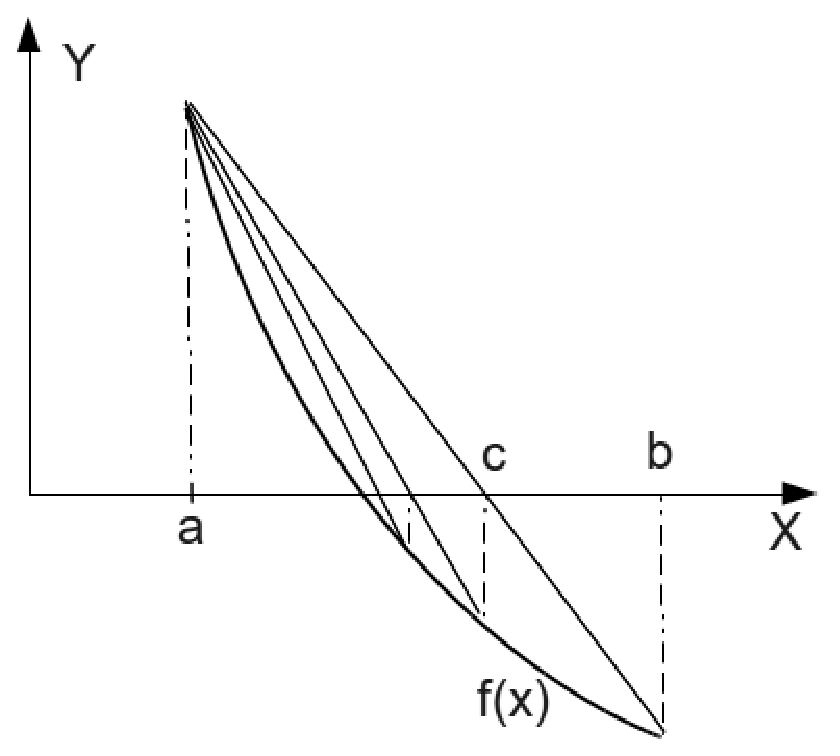
\includegraphics[width=0.5\textwidth]{img/ris_4_5}
\caption{Графическая интерпретация метода хорд}
\label{ch04:refDrawing4}
\end{center}
\end{figure}

Запишем уравнение прямой, проходящей через точки с координатами   $(a,f(a))$  и  $(b,f(b))$ :
\begin{equation}\label{ch04:refDrawing1a}
\frac{y-f(a)}{f(b)-f(a)}=\frac{x-a}{b-a},\ \ \  y=\frac{f(b)-f(a)}{b-a}\cdot (x-a)+f(a)
\end{equation}

Прямая, заданная уравнением (\ref{ch04:refDrawing1a}), пересекает ось $X$ при условии $y=0$.

Найдём точку пересечения хорды с осью $X$:\\
${y=\frac{f(b)-f(a)}{b-a}\cdot (x-a)+f(a)}$,\ \  ${x=a-\frac{f(a)\cdot (b-a)}{f(b)-f(a)}}$,\\ 
итак, \ \  ${c=a-\frac{f(a)}{f(b)-f(a)}(b-a)}$.

Далее необходимо вычислить значение функции в точке $c$. Это и будет приближённое значение корня
уравнения.

Для вычисления одного из корней уравнения  $x^2-\cos (5\cdot x)=0$  методом хорд достаточно знать интервал изоляции
корня, например,  $a=0.2;b=0.4$, и точность вычисления  $\varepsilon=10^{-3}$ . Блок-схема метода представлена на 
рис.~\ref{ch04:refDrawing5}. 

\begin{figure}[htb]
\begin{center}
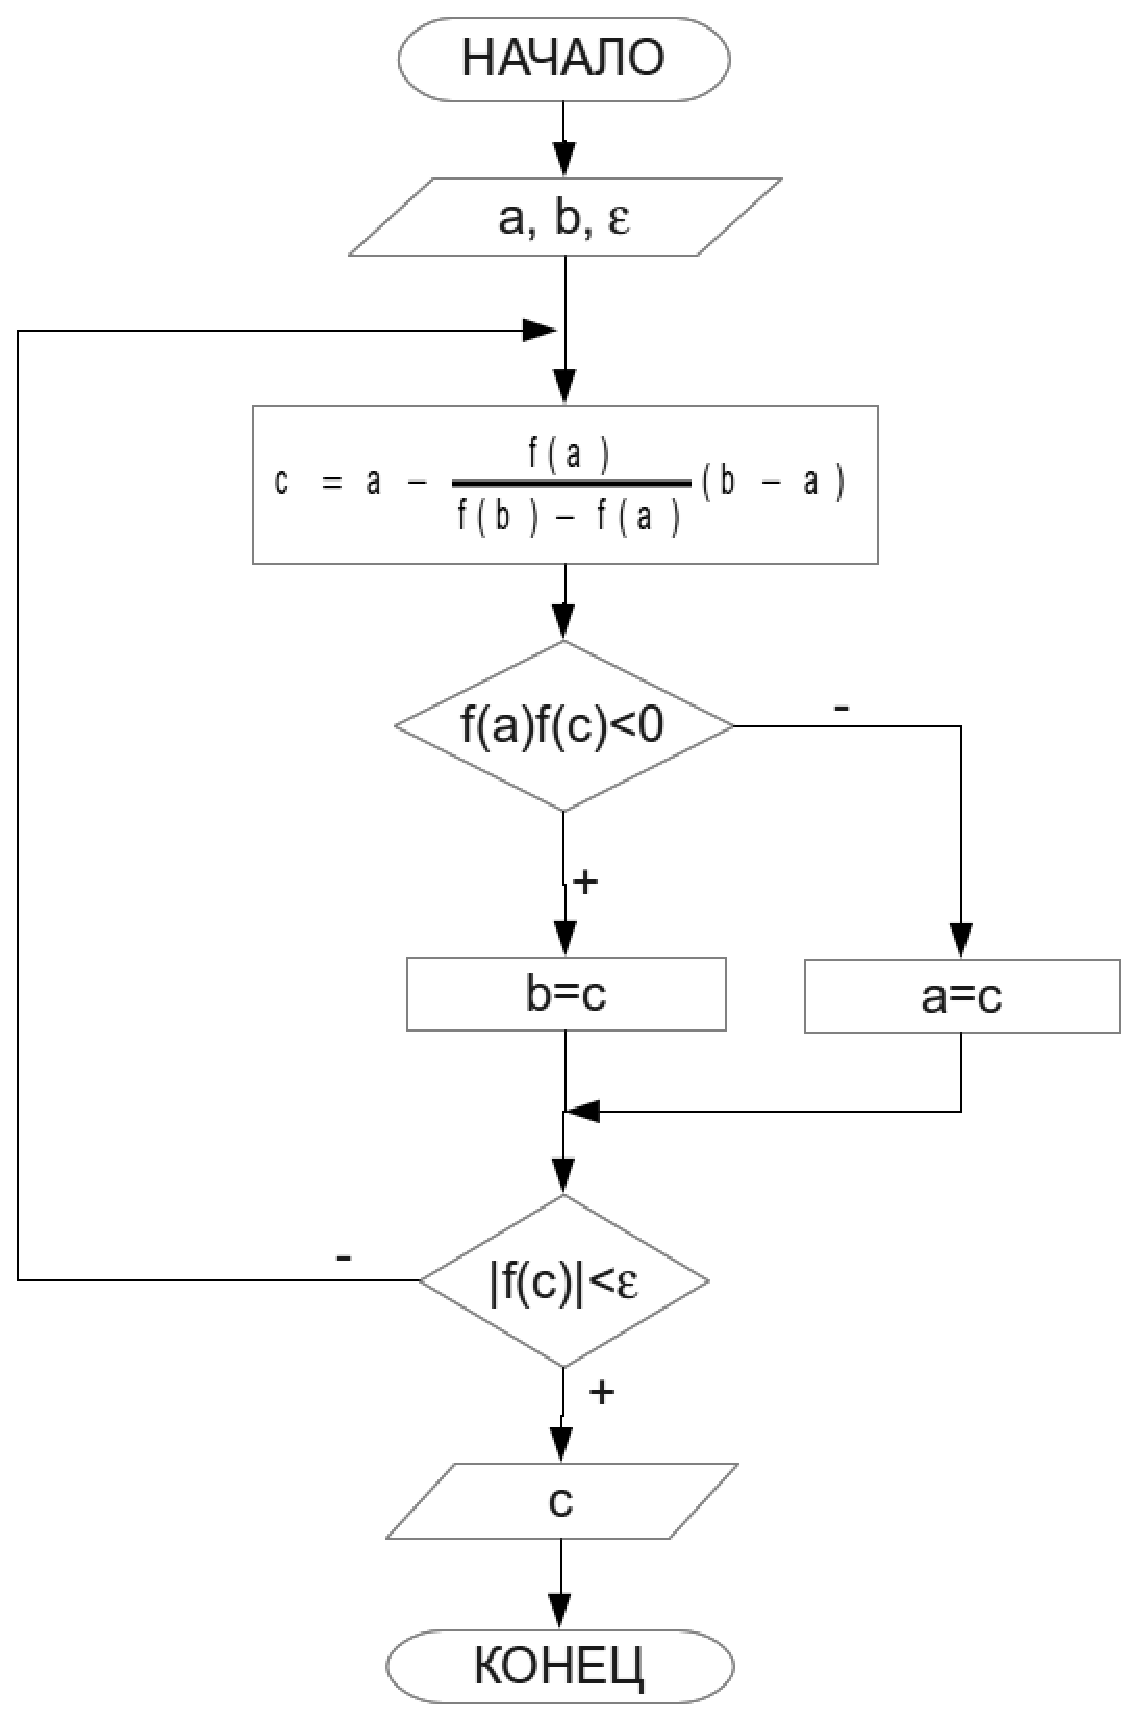
\includegraphics[width=0.5\textwidth]{img/ris_4_6}
\caption{Алгоритм метода хорд}
\label{ch04:refDrawing5}
\end{center}
\end{figure}

\emph{Метод касательных} (\emph{метод Ньютона}). В одной из точек интервала  $[a;b]$, пусть
это будет точка \emph{a}, проведём касательную (рис.~\ref{ch04:refDrawing6}). Запишем уравнение этой прямой:
\begin{equation}\label{ch04:refDrawing6a}
y=k\cdot x+m
\end{equation}

\begin{figure}[htb]
\begin{center}
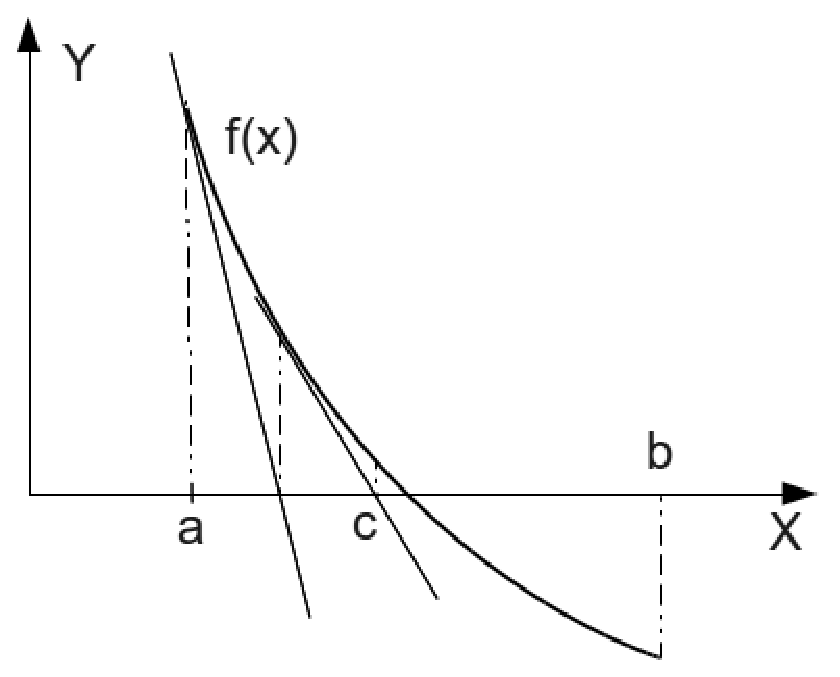
\includegraphics[width=0.5\textwidth]{img/ris_4_7}
\caption{Графическая интерпретация метода касательных}
\label{ch04:refDrawing6}
\end{center}
\end{figure}

Так как эта прямая является касательной, и она проходит через точку  $(c,f(c))$, то  $k=f'(c)$. 

Следовательно, 

$y=f'(x)\cdot x+m,f(c)=f'(c)\cdot c+m,m=f(c)-c\cdot f'(c),$

 $y=f'(c)\cdot x+f(c)-c\cdot f'(c),y=f'(c)\cdot (x-c)+f(c)$.

Найдём точку пересечения касательной с осью $X$:

 $f'(c)\cdot (x-c)+f(c)=0$,\ \ ${x=c-\frac{f(c)}{f'(c)}}$  

Если  $|f(x)|<\varepsilon$, то точность достигнута, и точка $x$ --- решение; иначе необходимо переменной
$c$ присвоить значение $x$ и провести касательную через новую точку
$c$; так продолжать до тех пор, пока  $|f(x)|$  не станет меньше  $\varepsilon$ . Осталось решить
вопрос, что выбрать в качестве точки начального приближения $c$.

В этой точке должны совпадать знаки функции и её второй производной. А так как нами было сделано допущение, что вторая и
первая производные не меняют знак, то можно проверить условие  $f(x)\cdot f''(x)>0$ на обоих 
концах интервала, и в качестве начального приближения взять ту точку, где это условие
выполняется.

Здесь, как и в предыдущих методах, для вычисления одного из корней уравнения  $x^2-\cos (5\cdot x)=0$  достаточно
знать интервал изоляции корня, например,  $a=0.2;b=0.4$,  и точность вычисления  $\varepsilon=10^{-3}$. Блок-схема
метода Ньютона представлена на рис. \ref{ch04:refDrawing7}. Понятно, что для реализации этого алгоритма нужно найти первую и
вторую производные функции  $f(x)=x^2-\cos (5\cdot x)$:  $f'(x)=2\cdot x+5\cdot \sin (5\cdot x)$ , 
$f(x) =2 +25 \cdot cos(5 \cdot x)$.

\begin{figure}[htb]
\begin{center}
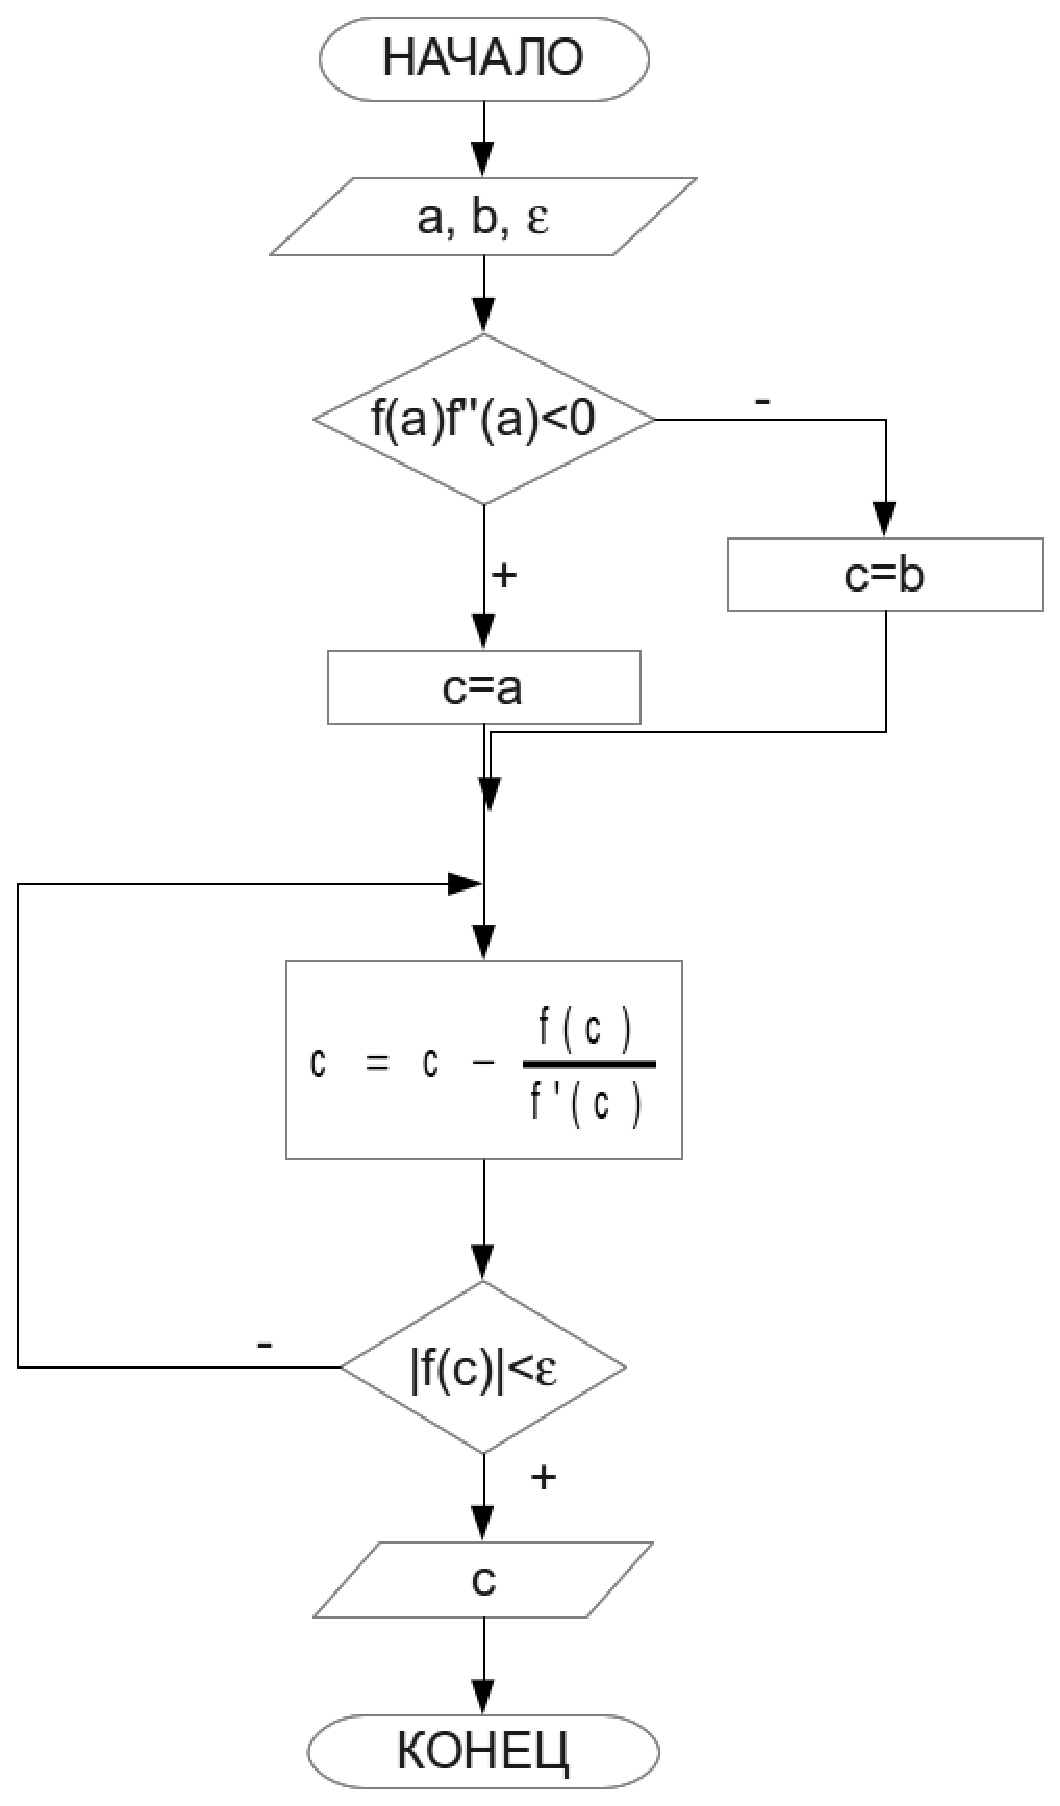
\includegraphics[width=0.5\textwidth]{img/ris_4_8}
\caption{Алгоритм метода Ньютона}
\label{ch04:refDrawing7}
\end{center}
\end{figure}

\emph{Метод простой итерации}. Для решения уравнения этим методом необходимо записать уравнение
(\ref{ch04:refDrawing0a}) в виде  $x=\phi(x)$, задать начальное приближение  $x_0\in [a;b]$ и организовать следующий
итерационный вычислительный процесс: 

$x_{k+1}=\phi(x_k),k=0,1,2,...$

Вычисление прекратить, если  $|x_{k+1}-x_k|<\varepsilon$
($\varepsilon$ --- точность).

Если неравенство  $|\phi'(x)|<1$ выполняется на всём интервале  $[a;b]$, то последовательность 
$x_0, x_1, x_2,...,x_n,...$ сходится к решению $x^*$ (т.е.$\lim\limits_{k\rightarrow \infty}x_k=x^*$).


Значение функции  $\phi(x)$  должно удовлетворять условию  $|\phi'(x)|<1$  для того, чтобы можно было применить метод
простых итераций. Условие  $|\phi'(x)|<1$  является
\emph{достаточным условием сходимости} метода простой итерации.

Уравнение (\ref{ch04:refDrawing0a}) можно привести к виду  $x=\phi(x)$ 
следующим образом. Умножить обе части уравнения  $f(x)=0$
на число  $\lambda$. К обеим частям уравнения  $\lambda\cdot f(x)=0$ добавить число $x$. Получим 
$x=x+\lambda\cdot f(x)$. Это и есть уравнение вида  $x=\phi(x)$, где 
\begin{equation}\label{ch04:refDrawing3a}
 \phi(x)=x+\lambda\cdot f(x)
\end{equation}

Необходимо чтобы неравенство  $|\phi'(x)|<1$ выполнялось на интервале  $[a;b]$, следовательно, 
$|\phi'(x)|=|1+\lambda\cdot f'(x)|$  и  $|1+\lambda\cdot f'(x)|<1$  ($|1+\lambda\cdot f'(a)|<1$,  $|1+\lambda\cdot
f'(b)|<1$), а значит, с помощью \emph{подбора параметра}  $\lambda$  можно добиться выполнения
\emph{условия сходимости}. 

Для вычисления корней уравнения  $x^2-\cos (5\cdot x)=0$  воспользуемся графическим 
решением (рис.~\ref{ch04:refDrawing1}) и
определим интервал изоляции одного из корней, например,  $a=0.2;b=0.4$. 
Подберём значение  $\lambda$,  решив
неравенство  $|1+\lambda\cdot f'(x)|<1$:
 
$|1+\lambda\cdot f'(a)|<1$ и  $|1+\lambda\cdot f'(b)|<1$,

$f(x)=x^{2}-\cos (5\cdot x),f'(x)=2\cdot x+5\cdot \sin (5\cdot x)$,

$f'(a)=2\cdot 0.2+5\cdot \sin (5\cdot 0.2)\approx 4.6$ ,  $f'(b)=2\cdot 0.4+5\cdot \sin (5\cdot 0.4)\approx 5.35$,

 $|1+\lambda\cdot 4.6|<1$  и  $|1+\lambda\cdot 5.35|<1$.

%Решим первое неравенство:
$$
\left\{\begin{array}{l}
\left\{\begin{array}{l}
1+4.6\cdot \lambda<1 \cr
1+4.6\cdot \lambda>-1
\end{array}\right.\cr
\left\{\begin{array}{l}
\lambda<0 \cr
\lambda>-0.37
\end{array}\right.
\end{array}\right.
\Rightarrow
\left\{\begin{array}{l}
\left\{\begin{array}{l}
\lambda<0 \cr
\lambda>-0.4
\end{array}\right.\cr
\left\{\begin{array}{l}
\lambda<0 \cr
\lambda>-0.37
\end{array}\right.
\end{array}\right.
\Rightarrow
\left\{\begin{array}{l}
\lambda\in (-0.4;0) \cr
\lambda\in (-0.37;0)
\end{array}\right.
$$

и, следовательно, 
$\lambda\in (-0.37;0)$.

Таким образом, исходными данными для программы будут начальное значение корня уравнения  $x_0=0.2$ , значение
параметра  $\lambda$ (пусть  $\lambda=-0.2$), и точность вычислений  $\varepsilon=0.001$ .

Для вычисления второго корня заданного уравнения параметр  $\lambda$  подбирают аналогично.

Блок-схема метода простой итерации приведена на рис.~\ref{ch04:refDrawing8}.
\begin{figure}[htb]
\begin{center}
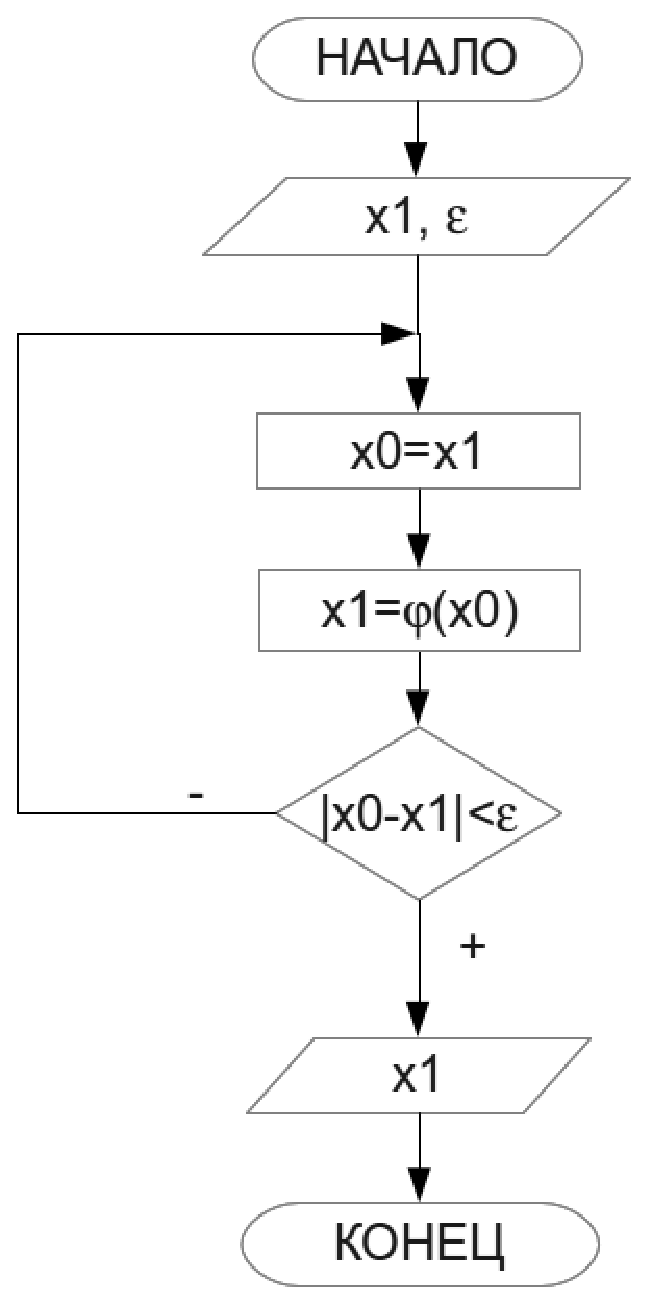
\includegraphics[width=0.5\textwidth]{img/ris_4_9}
\caption{Алгоритм метода простой итерации}
\label{ch04:refDrawing8}
\end{center}
\end{figure}

Далее представлен текст программы, реализующий решение задачи~\ref{ch04:prg7}.
\begin{lstlisting}
#include <iostream>
#include <math.h>
using namespace std;
//`Функция, определяющая левую часть уравнения $f(x)=0$.`
double f(double x)
{
  return(x*x-cos(5*x));
}
//`Функция, реализующая метод половинного деления.`
int Dichotomy(double a, double b, double *c, double eps)
{int k=0;
  do
  {
    *c=(a+b)/2;
    if (f(*c)*f(a)<0) b=*c;
    else a=*c;
    k++;
  }
  while (fabs(a-b)>=eps);
  return k;
}
//`Функция, реализующая метод хорд.`
int Chord(double a, double b, double *c, double eps)
{int k=0;
  do
  {
    *c=a-f(a)/(f(b)-f(a))*(b-a);
    if (f(*c)*f(a)>0) a=*c;
    else b=*c;
    k++;
  }
  while (fabs(f(*c))>=eps);
  return k;
}
double f1(double x)  //`Первая производная функции $f(x)$.`
{
  return(2*x+5*sin(5*x));
}
double f2(double x)  //`Вторая производная функции $f(x)$.`
{
  return(2+25*cos(5*x));
}
//`Функция, реализующая метод касательных.`
int Tangent(double a, double b, double *c, double eps)
{int k=0;
  if (f(a)*f2(a)>0) *c=a;
  else *c=b;
  do
  {
    *c=*c-f(*c)/f1(*c);
    k++;
  }
  while (fabs(f(*c))>=eps);
  return k;
}
double fi(double x,double L) //`Функция, заданная выражением~\ref{ch04:refDrawing3a}`.
{
  return(x+L*f(x));
}
//`Функция, реализующая метод простой итерации.`
int Iteration(double *x, double L, double eps)
{int k=0; double x0;
  do
  {
    x0=*x;
    *x=fi(x0,L);
    k++;
  }
  while (fabs(x0-*x)>=eps);
  return k;
}
int main()
{
  double A, B, X, P;
  double ep=0.001;  //`Точность вычислений.`
  int K;
  cout<<"a=";cin>>A;  //`Интервал изоляции корня.`
  cout<<"b=";cin>>B;
  cout<<"`\Sys{Решение уравнения}` x^2-cos(5*x)=0."<<endl;
  cout<<"`\Sys{Метод дихотомии:}`"<<endl;
  K=Dichotomy(A,B,&X,ep);
  cout<<"`\Sys{Найденное решение}` x="<<X;
  cout<<", `\Sys{количество итераций}` k="<<K<<endl;
  cout<<"`\Sys{Метод хорд:}`"<<endl;
  K=Chord(A,B,&X,ep);
  cout<<" `\Sys{Найденное решение}` x="<<X;
  cout<<", `\Sys{количество итераций}` k="<<K<<endl;
  cout<<"`\Sys{Метод касательных}`:"<<endl;
  K=Tangent(A,B,&X,ep);
  cout<<" `\Sys{Найденное решение}` x="<<X;
  cout<<", `\Sys{количество итераций}` k="<<K<<endl;
  cout<<"`\Sys{Метод простой итерации}`:"<<endl;
  X=A;
  cout<<"L=";cin>>P;
  K=Iteration(&X,P,ep);
  cout<<" `\Sys{Найденное решение}` x="<<X;
  cout<<", `\Sys{количество итераций}` k="<<K<<endl;
  return 0;
}
\end{lstlisting}
Результаты работы программы:
\begin{verbatim}
a=0.2
b=0.4
Решение уравнения x^2-cos(5*x)=0.
Метод дихотомии:
Найденное решение x=0.296094, количество итераций k=8
Метод хорд:
Найденное решение x=0.296546, количество итераций k=2
Метод касательных:
Найденное решение x=0.296556, количество итераций k=2
Метод простой итерации:
L=-0.2
Найденное решение x=0.296595, количество итераций k=3
\end{verbatim}


\section[Рекурсивные функции]{Рекурсивные функции}
Под \index{Рекурсия}\emph{рекурсией} в программировании понимают функцию, которая вызывает сама себя.
\index{Функция!рекурсивная}\emph{Рекурсивные функции} чаще всего используют для компактной реализации
рекурсивных алгоритмов. Классическими рекурсивными алгоритмами могут быть возведение числа в целую положительную
степень, вычисление факториала. С другой стороны, любой рекурсивный алгоритм можно реализовать без применения рекурсий.
Достоинством рекурсии является компактная запись, а недостатком --- расход памяти на повторные вызовы функций и передачу
параметров, существует опасность переполнения памяти.

Рассмотрим применение рекурсии на примерах~\cite{C,Shim}. %[7, 8].

\prg{Вычислить факториал числа $n$.}{ch04:prg8}

Вычисление факториала подробно рассмотрено в задаче~\ref{ch03:prg12} 
(рис.~\ref{ch03:refDrawing27}). Для решения этой задачи с применением рекурсии
создадим функцию \Sys{factoial}, алгоритм которой представлен на рис.~\ref{ch04:refDrawing9}. 

\begin{figure}[htb]
\begin{center}
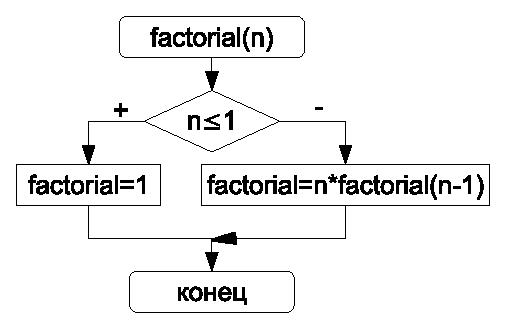
\includegraphics[width=0.5\textwidth]{img/ris_4_10}
\caption{Рекурсивный алгоритм вычисления факториала}
\label{ch04:refDrawing9}
\end{center}
\end{figure}


Текст программы с применением рекурсии:
\begin{lstlisting}
#include <iostream>
using namespace std;
long int factorial(int n)
{
  if (n<=1) 
    return n; 
  else 
  return n*factorial(n-1); 
}
int main()
{
  int i; long int f;
  cout<<"i="; cin>>i;
  f=factorial(i); 
  cout<<i<<"!="<<f<<"\n"; 
  return 0;
}
\end{lstlisting}

\prg{Вычислить $n$-ю степень числа $a$ ($n$ --- целое число).}{ch04:prg9}

Результатом возведения числа $a$ в целую степень $n$ является умножение этого числа
на себя $n$ раз. Но это утверждение верно только для положительных значений $n$.
Если $n$ принимает отрицательные значения, то  $a^{-n}=\frac{1}{a^n}$. В случае
$n=0$,  $a^0=1$.

Для решения задачи создадим рекурсивную функцию \Sys{stepen}, алгоритм которой 
представлен на рис.~\ref{ch04:refDrawing10}. 

\begin{figure}[htb]
\begin{center}
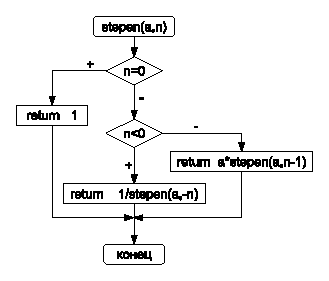
\includegraphics[width=0.5\textwidth]{img/ris_4_11}
\caption{Рекурсивный алгоритм вычисления степени числа}
\label{ch04:refDrawing10}
\end{center}
\end{figure}

Текст программы с применением рекурсии:
\begin{lstlisting}
#include <iostream> 
using namespace std;
float stepen(float a, int n) 
{
  if (n==0)
    return 1;
  else if (n<0) 
    return 1/stepen(a,-n); 
  else
    return a*stepen(a,n-1); 
}
int main()
{
  int i; float s,b;
  cout<<"b=";cin>>b;
  cout<<"i="; cin>>i;
  s=stepen(b,i);
  cout<<"s="<<s<<"\n"; 
  return 0;
}
\end{lstlisting}

\prg{Вычислить $n$-е число Фибоначчи.}{ch04:prg10}

Если нулевой элемент последовательности равен нулю, первый --- единице, а каждый последующий представляет собой сумму двух
предыдущих, то это \emph{последовательность чисел Фибоначчи} (0, 1, 1, 2, 3, 5, 8, 13, 21, 34, ... ). 

Алгоритм рекурсивной функции \Sys{fibonachi} изображён на рис.~\ref{ch04:refDrawing11}.

\begin{figure}[htb]
\begin{center}
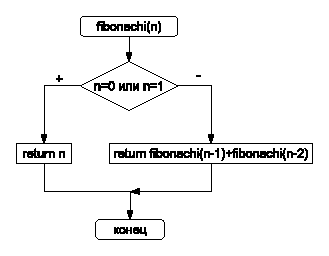
\includegraphics[width=0.5\textwidth]{img/ris_4_12}
\caption{Рекурсивный алгоритм вычисления числа Фибоначчи}
\label{ch04:refDrawing11}
\end{center}
\end{figure}

Текст программы:
\begin{lstlisting}
#include <iostream> 
using namespace std;
long int fibonachi(unsigned int n) 
{
  if ((n==0)||(n==1)) 
    return n; 
  else 
    return fibonachi(n-1)+fibonachi(n-2); 
}
int main()
{
  int i; long int f;
  cout<<"i="; cin>>i;
  f=fibonachi(i);
  cout<<"f="<<f<<"\n";
  return 0;
}
\end{lstlisting}

\section[Перегрузка функций]{Перегрузка функций}
Язык \Sys{C++} позволяет связать с одним и тем же именем функции различные определения, то есть возможно существование
нескольких функций с одинаковым именем. У этих функций может быть разное количество параметров или разные типы
параметров. Создание двух или более функций с одним и тем же именем называется \index{Функция!перегрузка
имени}\emph{перегрузкой имени функции}. Перегруженные функции создают, когда одно и то же действие следует
выполнить над разными типами входных данных.

В приведённом далее тексте программы три функции с именем \Sys{Pow}. Первая выполняет операцию возведения
вещественного числа $a$ в дробную степень  $n=\frac{k}{m}$, где $k$ и
$m$ --- целые числа. Вторая возводит вещественное число $a$ в целую степень
$n$, а третья --- целое число $a$ в целую степень\footnote{Как
известно, операция  $a^n$ не определена при $a=0$ и $n=0$, а так же при возведении
отрицательного значения $a$ в дробную степень  $n=\frac{k}{m}$, где $m$ --- чётное
число~(п.~\ref{ch02:7}).%(п.2.7). 
Пусть наши функции в этих случаях возвращают 0.} $n$. Какую именно функцию вызвать
компилятор определяет по типу фактических параметров. Так, если $a$ --- вещественное число, а
$k$ --- целое, то оператор \Sys{Pow(a,k)} вызовет вторую функцию, так как она имеет
заголовок \Sys{float Pow(float a, int n)}. Команда \Sys{Pow((int)a,k)} приведёт к вызову
третьей функции \Sys{float Pow(int a, int n)}, так как вещественная переменная $a$
преобразована к целому типу. Первая функция \Sys{float Pow(float a, int k, int m)} имеет три параметра,
значит, обращение к ней осуществляется командой \Sys{Pow(a,k,m)}. 
\begin{lstlisting}
#include <iostream> 
using namespace std;
#include <math.h> 
float Pow(float a, int k, int m) //`Первая функция`
{
  cout<<"`Функция` 1 \t"; 
  if (a==0) 
    return 0; 
  else if (k==0) 
        return 1; 
       else if (a>0) 
              return exp((float)k/m*log(a)); 
            else if (m%2!=0) 
              return -(exp((float)k/m*log(-a))); 
}
float Pow(float a, int n)  //`Вторая функция`
{
  float p; int i;
  cout<<"`Функция` 2 \t";
  if (a==0) 
    return 0; 
  else if (n==0) 
    return 1; 
    else if (n<0) 
    {
      n=-n;
      p=1;
      for(i=1;i<=n;i++)
        p*=a;
      return (float)1/p;
    }
      else 
      {
        p=1;
        for(i=1;i<=n;i++)
          p*=a;
        return p; 
      }
}
float Pow(int a, int n) //`Третья функция`
{
  int i,p;
  cout<<"`Функция` 3 \t";
  if (a==0) 
    return 0; 
  else if (n==0) 
    return 1; 
    else if (n<0) 
   {
     n=-n;
     p=1;
     for(i=1;i<=n;i++)
       p*=a;
     return (float)1/p;
   }
     else 
     {
       p=1;
       for(i=1;i<=n;i++)
         p*=a;
       return p; 
     }		
}
int main()
{
  float a; int k,n,m; 
  cout<<"a="; cin>>a; 
  cout<<"k="; cin>>k; 
  cout<<"s="<<Pow(a,k)<<"\n";      //`Вызов 2-й функции.`
  cout<<"s="<<Pow((int)a,k)<<"\n"; //`Вызов 3-й функции.`
  cout<<"a="; cin>>a; 
  cout<<"k="; cin>>k; 
  cout<<"m="; cin>>m; 
  cout<<"s="<<Pow(a,k,m)<<endl;    //`Вызов 1-й функции.`
  return 0;
}
\end{lstlisting}

Результаты работы программы: 
\begin{verbatim}
a=5.2 
k=3 
Функция 2 	s=140.608 
Функция 3 	s=125 
a=-8 
k=1 
m=1 
Функция 1 	s=-8 

a=5.2 
k=-3 
Функция 2 	s=0.00711197 
Функция 3 	s=0.008 
a=-8 
k=1 
m=3 
Функция 1 	s=-2 
\end{verbatim}


\section[Шаблоны функций]{Шаблоны функций}
\index{Функция!шаблон}\emph{Шаблон} --- это особый вид функции. С помощью шаблона функции можно определить
алгоритм, который будет применяться к данным различных типов. Механизм работы шаблона заключается в том, что на этапе
компиляции конкретный тип данных передаётся в функцию в виде параметра.

Простейшую функцию–шаблон в общем виде можно записать так~\cite{OOPz}:
\begin{lstlisting}
template <class Type> `\Sys{заголовок}`
{
  `\Sys{тело функции}`
}
\end{lstlisting}

Обычно в угловых скобках указывают список используемых в функции типов данных. Каждый тип предваряется служебным словом
\Sys{class}. В общем случае в списке могут быть не только типы данных, но и имена переменных.

Рассмотрим пример шаблона поиска наименьшего из четырёх чисел.
\begin{lstlisting}
#include <iostream> 
using namespace std;
//`Определяем абстрактный тип данных с помощью служебного слова` Type.
template <class Type>
Type minimum(Type a, Type b, Type c, Type d)
{ //`Определяем функцию с использованием типа данных` Type.
  Type min=a;
  if (b<min) min=b; 
  if (c<min) min=c; 
  if (d<min) min=d; 
  return min; 
}
int main()
{
  int ia,ib,ic,id,mini; float ra,rb,rc,rd,minr; 
  cout<<"Vvod 4 thelih chisla\t";
  cin>>ia>>ib>>ic>>id; 
  mini=minimum(ia,ib,ic,id); //`Вызов функции` minimum, `в которую передаём` 
                             //`4 целых значения.`
  cout<<"\n"<<mini<<"\n";
  cout<<"Vvod 4 vecshestvenih chisla\t"; cin>>ra>>rb>>rc>>rd; 
  minr=minimum(ra,rb,rc,rd); //`Вызов функции` minimum, `в которую  передаём` 
                             //`4 вещественных значения.`
  cout<<"\n"<<minr<<"\n"; 
  return 0;
}
\end{lstlisting}

\section[Область видимости переменных в функциях]{Область видимости переменных в функциях}
Как известно (п.~\ref{ch02:8}), по месту объявления переменные в языке \Sys{C++} делятся на три класса: локальные, глобальные и
переменные, описанные в списке формальных параметров функций. Все эти переменные имеют разную область видимости. 

\emph{Локальные переменные} объявляются внутри функции и доступны только в ней. О таких переменных говорят,
что они имеют локальную видимость, то есть, видимы только внутри функции. 

\emph{Глобальные переменные} описывают вне всех функций. Поскольку они доступны из любой точки программы,
то их область видимости охватывает весь файл.

Одно и тоже имя может использоваться при определении глобальной и локальной переменной. В этом случае в теле функции
локальная переменная имеет преимущество и <<закрывает>> собой глобальную. Вне этой функции <<работает>> глобальное описание
переменной.

Из функции, где действует локальное описание переменной, можно обратиться к глобальной переменной с таким же именем,
используя \emph{оператор расширения области видимости}

\Sys{::переменная;}

Рассмотрим пример:
\begin{lstlisting}
#include <iostream> 
using namespace std;
float pr=100.678; //`Переменная` pr `определена глобально.`
int prostoe (int n) 
{
  int pr=1,i; //`Переменная` pr `определена локально.`
  if (n<0) pr=0; 
  else 
    for (i=2;i<=n/2;i++) 
      if (n%i==0){pr=0;break;} 
  cout<<"local pr="<<pr<<"\n";  //`Вывод локальной переменной.`
  cout<<"global pr="<<::pr<<"\n";  //`Вывод глобальной переменной.`
  return pr; 
} 
int main()
{
  int g;
  cout<<"g="; cin>>g;
  if (prostoe(g)) cout<<"g - prostoe \n";
  else cout<<"g - ne prostoe \n";
  return 0;
}
\end{lstlisting}
Результаты работы программы:
\begin{verbatim}
g=7 
local pr=1 		//Локальная переменная.
global pr=100.678 	//Глобальная переменная.
g - prostoe 
\end{verbatim}

\section[Функция main(). Параметры командной строки]{Функция main(). Параметры командной строки}\label{ch04:9}
Итак, любая программа на \Sys{C++} состоит из одной или нескольких функций, причём одна из них должна обязательно носить
имя \Sys{main} (основной, \emph{главный}). Именно этой функции передаётся управление после
запуска программы. Как любая функция, \Sys{main} может принимать параметры и возвращать значения. У
функции \Sys{main} две формы записи: 

\begin{itemize}
\item без параметров:
\begin{lstlisting}
`\Sys{тип}` main() {`\Sys{тело функции}`},
\end{lstlisting}
\item и с двумя параметрами:
\begin{lstlisting}
`\Sys{тип}` main(int argc, char *argv[]) {`\Sys{тело функции}`}.
\end{lstlisting}
\end{itemize}

Первый параметр \Sys{argc} определяет количество параметров, передаваемых в функцию \Sys{main} из командной
строки. Второй параметр \Sys{argv} --- указатель на массив указателей типа
\Sys{char} (массив строк). Каждый элемент массива ссылается на
отдельный параметр командной строки. При стандартном запуске программы \Sys{argc} равно 1, 
\Sys{argv} --- массив из одного элемента,
этим элементом является имя запускаемого файла.

Рассмотрим следующую программу. 
\begin{lstlisting}
#include <iostream>
#include <stdlib.h>
using namespace std;
int main(int argc, char *argv[])
{
  int i;
  cout<<"`\Sys{В командной строке}` "<<argc<<" `\Sys{аргументов}`\n";
  for(i=0;i<argc;i++)
  cout<<"`\Sys{Аргумент №}` "<<i<<" "<<argv[i]<<endl;
  return 0;
}
\end{lstlisting}

Текст программы хранится в файле \Sys{1.cpp}. При стандартном запуске программа выведет следующую
информацию:
\begin{verbatim}
В командной строке 1 аргументов
Аргумент № 0 ./1
\end{verbatim}
Программа выводит количество параметров командной строки и последовательно все параметры. При стандартном запуске –
количество аргументов командной строки --- 1, этим параметром является имя запускаемого файла (в нашем случае, имя
запускаемого файла --- \Sys{./1}).

Запустим программу следующим образом: 

\Sys{./1 abc 34 6 + 90 Вася Маша}

Результаты работы программы представлены ниже.
\begin{verbatim}
В командной строке 8 аргументов 
Аргумент № 0 ./1 
Аргумент № 1 abc 
Аргумент № 2 34 
Аргумент № 3 6 
Аргумент № 4 + 
Аргумент № 5 90 
Аргумент № 6 Вася 
Аргумент № 7 Маша
\end{verbatim}

Рассмотрим приложение, в которое в качестве параметров командной строки 
передаётся \Sys{число1, операция, число2}. Функция выводит

\Sys{число1 операция число2}.

Текст программы приведён на ниже\footnote{Функция \Sys{atof} преобразовывает строку символов в вещественное число, а если
преобразование невозможно, то результатом функции \Sys{atof} будет число 0.0. Функция \Sys{strcmp} сравнивает две строки и
возвращает 0 в случае совпадения строк. Подробнее об этих функциях можно прочесть в главе, посвящённой строкам.}
\begin{lstlisting}
#include <iostream>
#include <stdlib.h>
#include <cstring>
using namespace std;
int main(int argc, char **argv)
{
//`Если количество параметров больше или равно 4, то были введены два числа и знак операции.`
  if (argc>=4)
//`Если операция $*$, то выводим число1$*$число2.`
  {
    if (!strcmp(argv[2],"*")) cout<<atof(argv[1])*atof(argv[3])<<endl;
    else
//`Если операция $+$, то выводим число1$+$число2.`
      if (!strcmp(argv[2],"+")) cout<<atof(argv[1])+atof(argv[3])<<endl;
      else 
//`Если операция $-$, то выводим число1$-$число2.`
        if (!strcmp(argv[2],"-")) cout<<atof(argv[1])-atof(argv[3])<<endl;
        else 
//`Если операция /, то выводим число1/число2.`
	  if (!strcmp(argv[2],"/")) cout<<atof(argv[1])/atof(argv[3])<<endl;
	  else cout<<"`\Sys{неправильный знак операции}`"<<endl;	
  }
  else
    cout<<"`\Sys{недостаточное количество операндов}`"<<endl;
  return 0;
}
\end{lstlisting}

Ниже приведены варианты запуска программы и результаты её работы\footnote{Текст программы хранится в файле
\Sys{4.cpp}. Имя исполняемого файла \Sys{./4} (ОС Lnux)}. Предлагаем читателю самостоятельно разобраться с
результатами всех тестовых запусков приложения.
\begin{verbatim}
./4 1.3 + 7.8 
9.1 
./4 1.3 - 7.8 
-6.5 
./4 1.3 / 7.8 
0.166667 
./4 1.3 \* 7.8 
10.14 
./4 1.3 % 7.8 
неправильный знак операции 
./4 1.3+ 7.8 
недостаточное количество операндов 
\end{verbatim}

\section[Задачи для самостоятельного решения]{Задачи для самостоятельного решения}
\subsection[Применение функций при работе с последовательностями чисел]{Применение функций при работе с
последовательностями чисел}
Разработать программу на языке \Sys{C++} для следующих заданий:

\begin{enumerate}
\item Вводится последовательность целых положительных чисел, 0 --- конец последовательности. Для каждого элемента
последовательности определить и вывести на экран число, которое получится после записи цифр исходного числа в обратном
порядке.
\item Вводится последовательность целых чисел, 0 --- конец последовательности. Определить, содержит ли последовательность
хотя бы одно\emph{ совершённое число}. Совершённое число равно сумме всех своих делителей, не
превосходящих это число. Например, $6=1+2+3$ или $28=1+2+4+7+14$.
\item Вводится последовательность из $N$ целых положительных элементов. Определить, содержит ли последовательность хотя бы
одно \emph{простое число}. Простое число не имеет делителей, кроме единицы и самого себя.
\item Вводится последовательность из $N$ целых положительных элементов. Посчитать количество чисел-\emph{палиндромов}. 
Числа-палиндромы симметричны относительно своей середины, например, 12021 или 454.
\item Вводится последовательность из $N$ целых положительных элементов. Подсчитать количество совершённых и простых чисел
в последовательности.
\item Поступает последовательность целых положительных чисел, 0 --- конец последовательности. Определить, в каком из чисел
больше всего делителей.
\item Поступает последовательность целых положительных чисел, 0 --- конец последовательности. Определить, в каком из чисел
больше всего цифр. 
\item Вводится последовательность из $N$ целых положительных элементов. Проверить, содержит ли последовательность хотя бы
одну пару соседних \emph{дружественных чисел}. Два различных натуральных числа являются дружественными,
если сумма всех делителей первого числа (кроме самого числа) равна второму числу. Например, 220 и 284, 1184 и 1210,
2620 и 2924, 5020 и 5564.
\item Поступает последовательность целых положительных чисел, 0 --- конец последовательности. 
Каждый элемент последовательности представляет собой номер $m$ одного из чисел Фибоначчи. 
Вычислить и вывести на экран \mbox{$m$-\emph{е}} \emph{число Фибоначчи}. Напомним, что в последовательности Фибоначчи 
каждое последующее число представляет собой сумму двух предыдущих (0, 1, 1, 2, 3, 5, 8, 13, 21, 34, \dots). 
Например, четвёртое число Фибоначчи равно 3, седьмое --- 13, а девятое --- 34.
\item Вводится последовательность из $N$ целых положительных элементов. Найти число с минимальным количеством цифр.
\item Вводится последовательность из $N$ целых элементов. Для всех положительных элементов последовательности вычислить
значение \emph{факториала}. Вывести на экран число и его факториал.
\item Поступает последовательность целых положительных чисел, 0 --- конец последовательности. Вывести на экран все числа
последовательности, являющиеся \emph{составными} и их делители. Составное число имеет более двух делителей,
то есть не является \emph{простым}.
\item Вводится последовательность из $N$ целых положительных элементов. Определить, содержит ли последовательность хотя бы
одно \emph{число Армстронга}. Число Армстронга --- натуральное число, которое равно сумме своих цифр,
возведённых в степень, равную количеству его цифр. Например, десятичное число 153 --- число Армстронга, потому что: 
$1^3+3^3+5^3=1+27+125=153.$ 
\item Поступает последовательность целых положительных чисел, 0 --- конец последовательности. Найти среднее арифметическое
\emph{простых} чисел в этой последовательности. Простое число не имеет делителей, кроме единицы и самого
себя.
\item Вводится последовательность из $N$ целых положительных элементов. Определить, сколько в последовательности пар
соседних \emph{взаимно простых чисел}. Различные натуральные числа являются взаимно простыми, если их
наибольший общий делитель равен единице.
\item В последовательности из $N$ целых положительных элементов найти сумму всех \emph{недостаточных чисел}.
Недостаточное число всегда больше суммы всех своих делителей за исключением самого числа.
\item Вводится последовательность из $N$ целых положительных элементов. Посчитать количество элементов последовательности,
имеющих в своём представлении цифру 0.
\item Вводится $N$ пар целых положительных чисел $a$ и $b$. В случае, если
$a>b$ вычислить:
 $C=\frac{a!}{b!\cdot (a-b)!}$.
\item Вводится последовательность из $N$ целых элементов. Для каждого элемента последовательности найти среднее значение
его цифр.
\item Вводится последовательность целых положительных чисел, 0 --- конец последовательности. Для каждого элемента
последовательности определить и вывести на экран число, которое получится, если поменять местами первую и последнюю
цифры исходного числа.
\item Вводится последовательность из $N$ целых элементов. Для каждого элемента последовательности вывести на экран
количество цифр и количество делителей.
\item Вводится последовательность из $N$ целых положительных элементов. Среди элементов последовательности найти
наибольшее число-\emph{палиндром}. Числа-палиндромы симметричны относительно своей середины, например,
12021 или 454.
\item Поступает последовательность целых положительных чисел, 0 --- конец последовательности. Для каждого элемента
последовательности вывести на экран сумму квадратов его цифр.
\item Вводится последовательность из $N$ целых положительных элементов. Для \emph{простых} элементов
последовательности определить сумму цифр. Простое число не имеет делителей, кроме единицы и самого себя.
\item Вводится последовательность целых положительных чисел, 0 --- конец последовательности. Среди элементов
последовательности найти наименьшее \emph{составное число}. Составное число имеет более двух делителей, то
есть не является \emph{простым}.
\end{enumerate}

\subsection[Применение функций для вычислений в различных системах счисления]{Применение функций для вычислений в
различных системах счисления}
Разработать программу на языке \Sys{C++} для решения следующей задачи. Заданы два числа --- $A$ и
$B$, первое в системе счисления с основанием $p$, второе в системе счисления с
основанием $q$. Вычислить значение $C$ по указанной формуле и вывести его на экран
в десятичной системе счисления и системе счисления с основанием $r$. Исходные данные для решения
задачи представлены в табл. \ref{ch04:refTable0}.

\noindent
\begin{longtable}{|c|c|c|c|c|}
\caption{Задания для решения задачи о различных системах счисления}\label{ch04:refTable0}\\
\hline
\Emph{Вариант}&\Emph{p}&\Emph{q}&\Emph{C}&\Emph{r}\\\hline\hline
\endfirsthead
\multicolumn{5}{c}%
{{\tablename\ \thetable{} --- продолжение}} \\
\hline
\Emph{Вариант}&\Emph{p}&\Emph{q}&\Emph{C}&\Emph{r}\\\hline \hline
\endhead
1 &2 &8 &$A^{2}\cdot (A+B)$ &3\\\hline
2 &3 &7 &$2\cdot (A^{2}+B^{2})$ &4\\\hline
3 &4 &6 &$2\cdot B^{2}\cdot (A+B)$ &5\\\hline
4 &5 &2 &$(A-B)^{2}+3\cdot A$ &6\\\hline
5 &6 &4 &$A^{2}+A\cdot B$ &7\\\hline
6 &7 &3 &$(5\cdot B-2\cdot A)^{2}$ &8\\\hline
7 &8 &2 &$(2\cdot A-3\cdot B)^{2}$ &5\\\hline
8 &3 &8 &$(B-A)^{2}+2\cdot A$ &6\\\hline
9 &4 &7 &$B^{3}-B^{2}+2\cdot A$ &2\\\hline
10 &5 &6 &$A^{3}-A^{2}+3\cdot B$ &8\\\hline
11 &6 &5 &$(2\cdot A-3\cdot B)^{2}$ &3\\\hline
12 &7 &4 &$A^{2}+2\cdot A+B^{2}$ &5\\\hline
13 &8 &3 &$A^{2}+3\cdot B+B^{2}$ &7\\\hline
14 &4 &2 &$A^{2}-2\cdot A+B$ &6\\\hline
15 &5 &8 &$3\cdot B^{2}-2\cdot B+A$ &3\\\hline
16 &6 &7 &$A^{2}+(B-A)^{2}$ &2\\\hline
17 &7 &6 &$3\cdot B^{2}+2\cdot A\cdot B$ &8\\\hline
18 &8 &5 &$2\cdot A^{2}+3\cdot A\cdot B$ &7\\\hline
19 &2 &4 &$B^{3}-2\cdot B+A$ &3\\\hline
20 &3 &8 &$A^{3}-2\cdot A+B$ &4\\\hline
21 &4 &7 &$(5\cdot A-2\cdot B)^{2}$ &5\\\hline
22 &5 &6 &$(B^{2}-3\cdot A)^{2}$ &7\\\hline
23 &6 &5 &$(A^{2}-2\cdot B)^{2}$ &8\\\hline
24 &7 &4 &$A^{2}\cdot B^{2}-A\cdot B$ &6\\\hline
25 &8 &3 &$A\cdot B+A^{2}-B$ &2\\\hline
\end{longtable}

\subsection[Применение функций для решения нелинейных уравнений]{Применение функций для решения нелинейных уравнений}
Разработать программу на языке \Sys{C++} для вычисления одного из корней уравнения  $f(x)=0$ методами, указанными в задании.
Для решения задачи предварительно определить интервал изоляции корня графическим методом. Вычисления проводить с
точностью  $\varepsilon=10^{-4}$. Оценить степень точности путём подсчёта количества итераций, выполненных для
достижения заданной точности. Исходные данные для решения задачи представлены в табл. \ref{ch04:refTable1}.

{\noindent\small\tabcolsep=0.3em
\begin{longtable}{|l|l|p{0.56\textwidth}|}
\caption{Задания к задаче о решении нелинейных уравнений} \label{ch04:refTable1}\\
\hline
\Emph{№}&\Emph{Уравнение $f(x)=0$}&\Emph{Методы решения}\\
\hline \hline
\endfirsthead
\multicolumn{3}{c}%
{{\tablename\ \thetable{} --- продолжение}} \\
\hline
\Emph{№}&\Emph{Уравнение $f(x)=0$}&\Emph{Методы решения}\\
\hline \hline
\endhead
1 &$x-0.2\cdot \sin (x+0.5)=0$ &метод половинного деления, метод хорд\\\hline
2 &$x^2-\lg(x+2)=0$ &метод касательных, метод простой итерации\\\hline
3 &$x^2-20\cdot \sin (x)=0$ &метод хорд, метод касательных\\\hline
4 &$\ln (x)+(x+1)^3=0$ &метод дихотомии, метод простой итерации\\\hline
5 &$x^2-\sin(5x)=0$ &метод половинного деления, метод касательных\\\hline
6 &$e^x+x^2-2=0$ &метод хорд, метод простой итерации.\\\hline
7 &$0.8\cdot x^{2}-\sin (10\cdot x)=0$ &метод половинного деления, метод хорд\\\hline
8 &$\sin (7\cdot x)+2\cdot x-6=0$ &метод касательных, метод простой итерации\\\hline
9 &$x\cdot \ln (x)-1=0$ &метод хорд, метод касательных\\\hline
10 &$2\cdot \lg(x)+0.5\cdot x=0$ &метод дихотомии, метод простой итерации\\\hline
11 &$e^{-x}-x^2=0$ &метод половинного деления, метод касательных\\\hline
12 &$x^2-3\cdot \cos (x^2)=0$ &метод хорд, метод простой итерации\\\hline
13 &$\sin (7\cdot x)-x^2+15=0$ &метод половинного деления, метод хорд\\\hline
14 &$(x-1)^2-0.5\cdot e^x=0$ &метод касательных, метод простой итерации\\\hline
15 &$2\cdot \ln (x)-0.2\cdot x+1=0$ &метод хорд, метод касательных\\\hline
16 &$2-x\cdot e^x=0$ &метод дихотомии, метод простой итерации\\\hline
17 &$0.1\cdot x^3+3\cdot x^2-10\cdot x-7=0$ &метод половинного деления, метод касательных\\\hline
18 &$0.1\cdot x^2-e^x=0$ &метод хорд, метод простой итерации\\\hline
19 &$e^{-2\cdot x}-2\cdot x+1=0$ &метод половинного деления, метод хорд\\\hline
20 &$x^2-3+0.5^x=0$ &метод касательных, метод простой итерации\\\hline
21 &$\lg(4\cdot x)-\cos (x)=0$ &метод хорд, метод касательных\\\hline
22 &$\ln(x)-\cos^2(x)=0$ &метод дихотомии, метод простой итерации\\\hline
23 &$\frac{4}{x}-0.2\cdot e^x=0$ &метод половинного деления, метод касательных\\\hline
24 &$\sqrt{x+6.5}-e^x=0$ &метод хорд, метод простой итерации.\\\hline
25 &$0.5^x+1-(x-2)^2=0$ &метод половинного деления, метод хорд\\\hline
\end{longtable}
}

